\documentclass[11pt,oneside]{book}
\usepackage{amsmath}
\usepackage{amssymb}
\usepackage{amsthm}
\usepackage{amsfonts}
\usepackage{multirow}
\usepackage{float}
\usepackage{diagbox}
\usepackage{xcolor}
\usepackage{caption}
\usepackage{graphicx}
\usepackage{subfigure}
\graphicspath{{img/}}
\usepackage{paralist}
\usepackage{tikz}
\let\itemize\compactitem
\let\enditemize\endcompactitem
\let\enumerate\compactenum
\let\endenumerate\endcompactenum
\let\description\compactdesc
\let\enddescription\endcompactdesc
\setlength{\parindent}{0pt}
\title{Notes of Mathematical Analysis}
\author{}
\date{}
\newtheorem{theorem}{Theorem}[section]
\newtheorem*{lemma}{Lemma}
\newtheorem{definition}{Definition}[section]
\theoremstyle{definition}
\newtheorem{ex}{Exercise}[section]
\newtheorem*{answer}{Answer}
\newcommand\thmref[1]{\textbf{Theorem \ref{#1}}}
\newcommand\figref[1]{\textbf{Figure \ref{#1}}}
\begin{document}
\newtheorem*{tips}{\emph{TIPS}}
\chapter{Groups}
\section{Logical Symbols}
The logical symbols are a kind of symbols using for theoretical statements.
    \begin{table}[H]
        \centering
        \caption{Frequently-used Logical Symbols}
        \begin{tabular}{|c|c|}\hline
            Symbols&Meanings\\\hline
            $L\Longrightarrow P$& Proposition $L$ is contained in proposition $P$\\
            $L \Longleftrightarrow P $&Proposition $L$ is equivalent to proposition $P$\\
            $\lnot P$&Not $P$\\
            $L\wedge P$&Proposition $L$ and proposition $P$\\
            $L \vee P$&Proposition $L$ or proposition $P$\\
            \hline
        \end{tabular}
    \end{table}
e.g.\[((A\Longrightarrow B)\wedge(\lnot B)\Longrightarrow (\lnot A) )\]


stands for `` if $A$ is contained in  $B$,and $B$ is not true,then $A$ is not true''.

We also call $ A \Longleftrightarrow B$ ``$A$ is the necessary and suffiecent condition of $B$''.

The typical math proposition is like ``$A\Longrightarrow B$''.In order to prove this proposition ,we can use the  implication relationship \[A\Longrightarrow C_1\Longrightarrow \cdots \Longrightarrow C_n\Longrightarrow B\]The every implication relationship in this chain is general truth or proved proposition.

\begin{table}[H]
    \centering
    \caption{Truth Table}
    \begin{tabular}{|c|c|c|c|}
        \hline
        \multirow{2}{*}{$\lnot A$}                       & $A$                    & 0         & 1             \\ \cline{2-4} 
                                                 & $\lnot A$            & 1            & 0             \\ \hline
        \multirow{3}{*}{$A \vee B$}                       &       \diagbox{$A$}{$B$}     &    0        &       1        \\ \cline{2-4} 
                                                 &          0       &   0         &        1        \\ \cline{2-4} 
                                                 &       1         &  1        &        1       \\ \hline
        \multirow{3}{*}{$A \wedge B$}                       &        \diagbox{$A$}{$B$}    &           0&        1          \\ \cline{2-4} 
                                                 &     0         &     0          &      0          \\ \cline{2-4} 
                                                 &        1        &                0       &    1       \\ \hline
        \multirow{3}{*}{$A\Longrightarrow B$}                      &  \diagbox{$A$}{$B$} & 0  &  1 \\ \cline{2-4} 
                                                & 0  &  1 &  1 \\ \cline{2-4} 
                                                & 1  &  0 & 1  \\ \hline
        \end{tabular}
    \end{table}
\begin{question}$\lnot (A\wedge B )\Leftrightarrow (\lnot A \vee \lnot B)$.
\end{question}
\begin{proof}
    (Use the truth table)

    If $A$ is ture, $B$ is ture, $A\wedge B$ is ture. $\lnot (A\wedge B)$ is false.$\lnot A $ is false,$\lnot B$ is false, $(\lnot A \vee \lnot B)$ is false.

    If $A$ is ture, $B$ is false, $A\wedge B$ is false. $\lnot (A\wedge B)$ is true.$\lnot A $ is false,$\lnot B$ is true, $(\lnot A \vee \lnot B)$ is ture.

    If $A$ is flase, $B$ is true, $A\wedge B$ is false. $\lnot (A\wedge B)$ is true.$\lnot A $ is true,$\lnot B$ is false, $(\lnot A \vee \lnot B)$ is ture.

    If $A$ is false, $B$ is false, $A\wedge B$ is false. $\lnot (A\wedge B)$ is true.$\lnot A $ is true,$\lnot B$ is true, $(\lnot A \vee \lnot B)$ is ture.

    So
    \[\lnot (A\wedge B )\Leftrightarrow (\lnot A \vee \lnot B)\]
\end{proof}    

\begin{question}
    $(A \Rightarrow B)\Leftrightarrow\lnot A \vee B$.
\end{question}
\begin{proof}
    Firstly, we confirm the truth of \[(A \Rightarrow B)\Rightarrow\lnot A \vee B\]

    If $(A \Rightarrow B)$ is false, then $\lnot A \vee B$ is true.

    If $(A \Rightarrow B)$ is ture ,then we have two posibilities. The first is $A$ is ture, $B$ is true, so $\lnot A \vee B$ is true. The second is $A$ is false,then $B$ can be true or false, but $\lnot A \vee B$ will be true.

    Hence, $(A \Rightarrow B)\Rightarrow\lnot A \vee B$.

    Secondly, we prove \[(A \Rightarrow B)\Leftarrow\lnot A \vee B\]

    If $\lnot A \vee B$ is false, then $(A \Rightarrow B)$ is true.

    If $\lnot A \vee B$ is true, we have
    \begin{enumerate}
        \item $\lnot A$ is true, $B$ is false, then, $A$ is false, $(A \Rightarrow B)$ is true.
        \item $\lnot A$ is false, $B$ is true, then, $A$ is true, $(A \Rightarrow B)$ is true.
        \item $\lnot A$ is true, $B$ is true, then, $A$ is false, $(A \Rightarrow B)$ is true.
    \end{enumerate}

    So $(A \Rightarrow B)\Leftarrow\lnot A \vee B$.
\end{proof}



\section{Homomorphisms and subgroups}
\begin{ex}
    If $f: G \to H$ is a homomorphism of groups, then $f(e_G) = e_H$ and $f(a^{-1}) = f(a)^{-1}$ for all $a \in G$. Show by example that the first conclusion may be false if $G$, $H$ are monoids that are not groups.
\end{ex}

$$ $$

\begin{ex}
    A group $G$ is abelian if and only if the map $G\to G$ given by $x\to x^{-1}$ is automorphism.
\end{ex}

$$ $$

\begin{ex}
    Let $Q_8$ be the group(under ordinary matrix multiplication) generated by complex matrices $A = \begin{pmatrix}
        0 & 1 \\
        -1 & 0
    \end{pmatrix}$ and $B = \begin{pmatrix}
        0 & i\\
        i & 0
    \end{pmatrix}$, where $i^{2}=-1$. Show that $Q_8$ is a nonabelian group of order 8. $Q_8$ is called the quaternion group.
\end{ex}

$$ $$

\begin{ex}
    Let $H$ be the group(under ordinary matrix multiplication) of real matrices generated by $C = \begin{pmatrix}
        0 & 1\\
        -1 & 0
    \end{pmatrix}$ and $D = \begin{pmatrix}
        0 & 1\\
        1 & 0
    \end{pmatrix}$. Show that $H$ is a nonabelian group of order 8 which is not isomorphic to the quaternion group, but is isomorphic to the group $D_4^*$.
\end{ex}

$$ $$

\begin{ex}
    Let $S$ be a nonempty subset of a group $G$ and define a relation on $G$ by $a ~ b$ if and only if $ab^{-1}\in S$. Show that $~$ is an equivalence relation if and only if $S$ is a subgroup of $G$.
\end{ex}

$$ $$

\begin{ex}
    A nonempty finte subset of a group is s subgroup if and only if it is closed under the product in $G$.
\end{ex}

$$ $$

\begin{ex}
    If $n$ is a fixed integer, then $\{kn | n\in \mathbf{Z}\}\subset\mathbf{Z}$ is an additive subgroup of $\mathbf{Z}$, which is isomorphic to $\mathbf{Z}$. 
\end{ex}

$$ $$

\begin{ex}
    The set $\{\sigma\in S_n | \sigma(n) = n\}$ is a subgroup of $S_n$ which is isomorphic to $S_{n-1}$.
\end{ex}

$$ $$

\begin{ex}
    Let $f: G\to H$ be a homomorphism of groups, $A$ a subgroup of $G$, and $B$ a subgroup of $H$.
    \begin{enumerate}
        \item $\mathrm{Ker} f$ and $f^{-1}(B)$ are subgroups of $G$.
        \item $f(A)$ is a subgroup of $H$.
    \end{enumerate}
\end{ex}

$$ $$

\begin{ex}
    List all subgroups of $Z_2\oplus Z_2$. Is $Z_2\oplus Z_2$ isomorphic to $Z_4$?
\end{ex}

$$ $$

\begin{ex}
    If $G$ is a subgroup, then $C = \{a\in G| ax = xa \text{ for all } x\in G\}$ is a abelian subgroup of $G$. $C$ is called the center of $G$.
\end{ex}

$$ $$

\begin{ex}
    The group $D_4^*$ is not cyclic, but can be generated by two elements. The same is true of $S_n$(nontrivial). What is the minimal number of generators of the additive group $\mathbf{Z}\oplus\mathbf{Z}$?
\end{ex}

$$ $$

\begin{ex}
    If $G = \left\langle a \right\rangle $ is a cyclic group and $H$ is any group, then every homomorphism $f:G\to H$ is completely determined by the element $f(a)\in H$.
\end{ex}

$$ $$

\begin{ex}
    The following cyclic subgroups are all isomorphic: the multiplication group $\left\langle i \right\rangle$ in $\mathbf{C}$, the additive group $\mathbf{Z_4}$ and the subgroup $\left\langle \begin{pmatrix}
        1 & 2 & 3 & 4\\
        2 & 3 & 4 & 1
    \end{pmatrix}\right\rangle$ of $S_4$.
\end{ex}

$$ $$

\begin{ex}
    Let $G$ be a group and $\mathrm{Aut} G$ is the set of all automorphisms of $G$.
    \begin{enumerate}
        \item $\mathrm{Aut} G$ is a group with composition of functions as binary operation.
        \item $\mathrm{Aut} \mathbf{Z}\cong Z_2$ and $\mathrm{Aut} Z_6 \cong Z_2$; $\mathrm{Aut} Z_8\cong Z_2\oplus Z_2$; $\mathrm{Aut} Z_p\cong Z_{p-1}$ ($p$ prime).
        \item What is $\mathrm{Aut Z_n}$ for arbitrary $n\in \mathbf{N^*}$?
    \end{enumerate}
\end{ex}

$$ $$

\begin{ex}
    For each prime $p$ the additive subgroup $Z(p^\infty)$ of $\mathbf{Q}/\mathbf{Z}$ is generated by the set $\{\bar{1/p^n}|n\in \mathbf{N^*}\}$.
\end{ex}

$$ $$

\begin{ex}
    Let $G$ be an abelian group and let $H, K$ be subgroups of $G$. Show that the join $H\vee K$ is the set $\{ab|a\in H, b\in K\}$. Extend this result to any finite number of subgroups of $G$.
\end{ex}

$$ $$

\begin{ex}
    \begin{enumerate}
        \item Let $G$ be a group and $\{H_i| i\in I\}$ a family of subgroups. State and prove a condition that will imply that $\bigcup\limits_{i\in I}H_i$ is a subgroup, that is $\bigcup\limits_{i\in I}H_i = \left\langle\bigcup\limits_{i\in I}H_i\right\rangle$.
        \item Given an example of a group $G$ and a family of subgroups $\{H_i|i \in I\}$ such that $\bigcup\limits_{i\in I}H_i \neq \left\langle\bigcup\limits_{i\in I}H_i\right\rangle$.
    \end{enumerate}
\end{ex}

$$ $$

\begin{ex}
    \begin{enumerate}
        \item The set of all subgroups of a group $G$, partially ordered by set theoretic inclusion, forms a complete lattice in which the g.l.b of $\{H_i|i\in I\}$ is $\bigcap\limits_{i\in I}H_i$ and the l.u.b is $\left\langle\bigcap\limits_{i\in I}H_i\right\rangle$.
        \item Exhibit the lattice of subgroups of the groups $S_3, D_4^*, Z_6, Z_{27}$ and $Z_{36}$.
    \end{enumerate}
\end{ex}
\section{Cyclic groups}
\begin{ex}
    Let $a,b$ be elements of group $G$. Show that $\left| a \right| =\left| a^{-1} \right| $; $\left| ab \right| =\left| ba \right| $, and $\left| a \right| =\left| cac^{-1} \right| $ for all $c\in G$.
\end{ex}

\begin{answer}
    We only consider that $\left| a \right| , \left| b \right| , \left| c \right| $ are finite. Assume $a^{k}=e$, $(ab)^{m}=e$, $(ac^{-1})^{n}=e$, $kmn\neq 0$. $a^{k}\cdot(a^{-1})^{k}=e$, so $k$ sialso the order of $a^{-1}$, $\left| a^{-1} \right| =k$. $(ab)^{m}=e=a(ba)^{m-1}b\Rightarrow (ba)^{m-1}=a^{-1}b^{-1}$, $(ba)^{m}=a^{-1}b^{-1}ba=e$. $m$ is the order of $ba$. $(cac^{-1})^{r}=cac^{-1}cac^{-1}\cdots cac^{-1}=ca^{n}c^{-1}=e$, so $a^{n}=e$, whence $n=k$.
\end{answer}

$$ $$

\begin{ex}
    Let $G$ be an abelian group containing elements $a$ and $b$ of orders $m$ and $n$ respectively. Show that $G$ contains an element whose order is the least commom multiple of $m$ and $n$.
\end{ex}

\begin{answer}
    If $(m,n)=1$, we know that $\forall a^{i}, i=1,2,\dots, m$, $b^{j}, j=1, 2, \dots, n$, $a^{i}b^{j}\neq e$, since if $a^{i}=b^{j}$, $\left| a^{i} \right| =n=\left| b^{-j} \right| =\left| b^{j} \right| =m$. $G$ is abelian, so $(ab)^{k}=a^{k}b^{k}\Rightarrow \left| ab \right|=mn=\left[ m,n\right]$.

    If $m|n$ or $n|m$, then $a$ or $b$ is the element we want. We consider $m|\!\!/n$ and $n|\!\!/m$. Factorise $n=p_{1}^{t_{1}}p_{2}^{t_{2}}\cdots p_{l}^{t_{l}}$, $m=p_{1}^{s_{1}}p_{2}^{s_{2}}\cdots p_{l}^{s_{l}}$, where $p_{1},\cdots,p_{l}$ are primes and $t_{1},\cdots,t_{l}, s_{1},\cdots, s_{l}\geq 0$. We can choose a new arrangement of $p_{1},\cdots,p_{l}$ and make $t_{1}\geq s_{1}$, $t_{2}\geq s_{2}$,\dots, $t_{i}\geq s_{i}$, $t_{i+1}<s_{i+1}$,\dots, $t_{l}<s_{l}$.\[(m,n)=p_{1}^{s_{1}}\cdots p_{i}^{s_{i}}p_{i+1}^{t_{i+1}}\cdots p_{l}^{t_{l}}, \left[m,n\right]=p_{1}^{t_{1}}\cdots p_{i}^{t_{i}}p_{i+1}^{s_{i+1}}\cdots p_{l}^{s_{l}}\] Take $x=a^{{p_{i+1}^{s_{i+1}}}\cdots p_{l}^{s_{l}}}$, $y=b^{{p_{1}^{t_{1}}}\cdots p_{i}^{t_{i}}}$, then $\left| x \right| ={p_{1}^{t_{1}}}\cdots p_{i}^{t_{i}}$, $\left| y \right| =p_{i+1}^{s_{i+1}}\cdots p_{l}^{s_{l}}$. Thus $(x,y)=1$, the order of $xy$ is $\left| x \right| \cdot\left| y \right| =p_{1}^{t_{1}}\cdots p_{i}^{t_{i}}p_{i+1}^{s_{i+1}}\cdots p_{l}^{s_{l}}=\left[m,n\right]$.
\end{answer}

$$ $$

\begin{ex}
    Let $G$ be an abelian group of order $pq$, with $(p,q)=1$. Assume there exist $a,b\in G$ such that $\left| a \right| =p, \left| b \right| =q$ and show that $G$ is cyclic.
\end{ex}

\begin{answer}
    From \textbf{Exercise 1.3.2} we know $a^{i}b^{j}\neq e$ for $i<p$, $j<q$. $\left| G \right| =pq$ for all $a^{i}b^{j}$ and $a^{m}b^{n}$ with $i\neq m$, $b\neq n$, $a^{i}b^{j}\neq a^{m}b^{n}$. So $G$ can be generated by $ab$. $G$ is cyclic.
\end{answer}

$$ $$

\begin{ex}
    If $f:G\to H$ is a homomorphism, $a\in G$, and $f(a)$ has finte order in $H$, then $\left| a \right| $ is infinite or $\left| f(a) \right| $ divides $\left| a \right| $.
\end{ex}

\begin{answer}
    Assume $\left| f(a) \right| =n$, $\left| a \right| =m$, and $n|\!\!/m$. Trivially, $m\geq n$. Assume $\gcd(m,n)=k\leq n$. $a^{m}=e\Rightarrow f(a)^{m}=e'=f(a)^{n}$. By Bezout theorem $\exists x,y\in \mathbf{Z}$ s.t. $f(a)^{mx+ny}=f(a)^{k}=e'$, $k\leq n$, that's contradictory!
\end{answer}

$$ $$

\begin{ex}
    Let $G$ be the multiplicative group of all nonsingular $2\times 2$ matrices with rational entries. Show that $a=\begin{pmatrix}
        0 & -1\\1 & 0
    \end{pmatrix}$has order 4 and $b=\begin{pmatrix}
        0& 1\\-1&-1
    \end{pmatrix}$has order 3, but $ab$ has infinite order. Conversely, show that the additive group $Z_{2}\oplus \mathbf{Z}$ contains nonzero elements $a,b$ of infinite order such that $a+b$ has finite order. 
\end{ex}

\begin{answer}
    The verification of $\left| a \right| =4$ and $\left| b \right| =3$ is trivial. $ab=\begin{pmatrix}
        1 & 1\\ 0& 1
    \end{pmatrix}$ $\det(ab=\lambda I)=0\Rightarrow \lambda_{1}=\lambda_{2}=1$. $ab$ is not diagnizable. By induction, we have $(ab)^{n}=\begin{pmatrix}
        1 & 2^{n-1}\\ 0& 1
    \end{pmatrix}$ which means $(ab)$ has infinite order.

    For $a=(\bar{0},1), b=(\bar{0},-1)\in Z_{2}\oplus\mathbf{Z}$, $a,b$ have infinite order, but $a+b=(\bar{0},0)$ has finite order 1.
\end{answer}

$$ $$

\begin{ex}
    If $G$ is a cyclic group of order $n$ and $k| n$, then $G$ has exactly one subgroup of order $k$.
\end{ex}

\begin{answer}
    Assume $a^{n}=e$, $mk=n$, we verify that $\left\langle a^{m}\right\rangle$ is a subgroup of order $k$. $\forall x,y\in \mathbf{Z}_{+}$, $a^{xm}\cdot a^{-ym}=a^{(x-y)m}\in \left\langle a^{m}\right\rangle$, so $\left\langle a^{m}\right\rangle$ is a subgroup. $a^{km}=e$, $a^{sm}\neq e$ for $s<k$, so $\left| \left\langle a^{m}\right\rangle \right| =k$.
\end{answer}

$$ $$

\begin{ex}
    Let $p$ be prime and $H$ a subgroup of $Z(p^{\infty})$.
    \begin{enumerate}[(a)]
        \item Every element of $Z(p^{\infty})$ has finite order $p^{n}$ for some $n\geq 0$.
        \item If at least one element of $H$ has order $p^{k}$ and no element of $H$ has order greater than $p^{k}$, then $H$ is the cyclic subgroup generated by $\bar{1/p^{k}}$, whence $H\cong Z_{p^{k}}$.
        \item If there is no upper bound on the orders of elements of $H$, then $H=Z(p^{\infty})$.
        \item The only proper subgroups of $Z(p^{\infty})$ are the finite cyclic groups $C_{n}=\left\langle\bar{1/p^{n}}\right\rangle\,(n=1,2,\dots)$. Futhermore, $\left\langle0\right\rangle=C_{0}<C_{1}<C_{2}<C_{3}<\cdots$.
        \item Let $x_{1},x_{2},\dots$ be elements of an abelian group $G$ such that $\left| x_{1} \right| =p, px_{2}=x_{1},px_{3}=x_{2},\dots,px_{n+1}=x_{n},\dots$. The subgroup generated by the $x_{i}(i\geq 1)$ is isomorphic to $Z(p^{\infty})$. 
    \end{enumerate}
\end{ex}

\begin{answer}
    \begin{enumerate}[(a)]
        \item $\forall  x\in Z(p^{\infty})$, $x=\frac{a}{p^{n}}$ where $a<p^{n}$, $p|\!\!/a$. $p$ is a prime, so $\gcd(p,a)=1$. $m\cdot a|p^{n}\Rightarrow m=p^{n}$. Thus $m\cdot \frac{a}{p^{n}}=e$, $p^{n}$ is the smallest number satisfies it. $\frac{a}{p^{n}}$ has order $p^{n}$.
        \item For all $x\in Z(p^{\infty})$, if $x$ has order smaller than $p^{k}$, $x$ must have the form $x=\frac{a}{p^{i}}(i\leq k)$, $(p,a)=1$, so $x\in\left\langle\frac{1}{p^{k}}\right\rangle$. If not, assume $x=\frac{a}{p^{i}}(i>k)$, then $p^{k}\cdot x=\frac{a}{p^{i-k}}\neq 1$.
        \item Assume not, $H< Z(p^{\infty})$, $H\neq Z(p^{\infty})$. There exist $y\in H$ s.t. $y$ has order $p^{m}, m\geq n$. $y=\frac{b}{p^{m}}$, $(p,b)=1$, so there exists $b^{-1}\in\{1,2,\dots,p-1\}$, $bb^{-1}\equiv 1\mod p^{m}$. But $ab^{-1}p^{m-n}y=\frac{a}{p^{n}}=x\in H$, that's contradictory! Conversely, $H=Z(p^{\infty})$.
        \item From (b), we know that if there's least upper bound $p^{n}$ for elements in a subgroup $S$, then $S=C_{n}$.\[\left\langle0\right\rangle=C_{0}<C_{1}<C_{2}<C_{3}<\cdots<Z(p^{\infty})\] is easy to verify.
        \item We can verify that $f:x_{i}\mapsto \bar{\frac{1}{p^{i}}}$ is a well defined isomorphism. $f(e)=f(px_{1})=1$, $f(px_{i+1})=f(x_{i})=\frac{1}{p^{i}}=p\cdot \frac{1}{p^{i+1}}$. $f$ is obviously a bijection, so $H\cong Z(p^{\infty})$.
    \end{enumerate}
\end{answer}

$$ $$

\begin{ex}
    A group that has only a finite number of subgroups must be finite.
\end{ex}

\begin{answer}
    Suppose not. If the order of all subgroups are finite, $G$ must be finite. So there exists a infinite subgroup $H<G$. $\forall  a\in G$, if $\forall n\in \mathbf{N}$, $a^{n}\neq e$. then we can construct infinte subgroups $\left\langle a\right\rangle$, $\left\langle a^{2}\right\rangle$, $\left\langle a^{3}\right\rangle$\dots. If $\forall a\in G$, $\exists n\in \mathbf{N}$, $a^{n}=e$, so $\left\langle a\right\rangle$ is a proper subgroup of $G$, we can take $b\in G\backepsilon\left\langle a\right\rangle$ to construct another subgroup. By induction, there are infinte subgroups in $G$. That's contradictory, so $G$ must be finite.
\end{answer}

$$ $$

\begin{ex}
    If $G$ is an abelian group, then the set $T$ of all elements of $G$ with finite order is a subgroup of $G$.
\end{ex}

\begin{answer}
    We can easily verify that $\forall a,b\in S$, $\left| a \right| =m$, $\left| b \right| =n$ and $\left| ab^{-1} \right| \leq mn$ is finite. $T$ is a subgroup of $G$.
\end{answer}

$$ $$

\begin{ex}
    An infinite group is cyclic if and only if it is isomorphic to each of its proper subgroups.
\end{ex}

\begin{answer}
    If $G$ is cyclic, $G\cong \mathbf{Z}$, $S<G$. For any subgroup of $\mathbf{Z}$, it has the form $\{na\}, a\in \mathbf{Z}$. We can construct a isomorphism $f:n\mapsto na$, so $S\cong \{na\}\Rightarrow G\cong S$.

    If $\forall S<G$, $G\cong S$ and $\left| G \right| =\left| S \right| $ is finite. We prove there exists $S<G$ s.t. $\left| S \right| =\aleph_{0}$. Take $a\in G$ and $S=\{na|n\in \mathbf{Z}\}$, $S$ is a subgroup. If there exists $ma=0$, $S$ must be finite, contradictory! Thus, $S\cong \mathbf{Z}\cong G$. $G$ is a infinite cyclic group.
\end{answer}
\section{Cosets and counting}
\begin{ex}
    Let $G$ be a group and $\{H_{i}|i\in I\}$ a family of subgroups. Then for any $a\in G$, $(\bigcap\limits_{i}H_{i})a=\bigcap\limits_{i}H_{i}a$.
\end{ex}

$$ $$

\begin{ex}
    \begin{enumerate}[(a)]
        \item Let $H$ be the cyclic subgroup (of order 2) of $S_{3}$ generated by $\begin{pmatrix}
            1 & 2 &3\\2& 1&3
        \end{pmatrix}$. Then no left cosets of $H$ (except $H$ itself) is also a right coset. There exists $a\in S_{3}$ such that $aH\cap Ha=\{a\}$.
        \item If $K$ is the cyclic subgroup (of order 3) of $S_{3}$ generated by $\begin{pmatrix}
            1 & 2&3\\2& 3 &1
        \end{pmatrix}$, then every left coset of $K$ is also a right coset of $K$.
    \end{enumerate}
\end{ex}

$$ $$

\begin{ex}
    The following conditions on a finite group $G$ are equivalent.
    \begin{enumerate}[(i)]
        \item $\left| G \right| $ is prime.
        \item $G\neq \left\langle e\right\rangle$ and $G$ has no proper subgroups.
        \item $G\cong Z_{p}$ for some prime $p$.
    \end{enumerate}
\end{ex}

$$ $$

\begin{ex}
    Let $a$ be an integer and $p$ be a prime such that $p\nmid a$. Then $a^{p-1}\equiv 1\mod p$.
\end{ex}

$$ $$

\begin{ex}
    Prove that there are only two distinct groups of order 4 (up to isomorphism), namely $Z_{4}$ and $Z_{2}\oplus Z_{2}$.
\end{ex}

$$ $$

\begin{ex}
    Let $H,K$ be subgroups of a group $G$. Then $HK$ is a subgroup of $G$ if and only if $HK=KH$.
\end{ex}

$$ $$

\begin{ex}
    Let $G$ be a group of order $p^{k}m$, with $p$ prime and $(p,m)=1$. Let $H$ be a subgroup of order $p^{k}$ and $K$ a subgroup of order $p^{d}$, with $0<d\leq k$ and $K\not\subset H$. Show that $HK$ is not a subgroup of $G$.
\end{ex}

$$ $$

\begin{ex}
    If $H$ and $K$ are subgroups of finite index of a group $G$ such that $\left[G:H\right]$ and $\left[G:K\right]$ are relatively prime, then $G=HK$.
\end{ex}

$$ $$

\begin{ex}
    If $H,K$ and $N$ are subgroups of a group $G$ such that $H<N$, then $HK\cap N=H(K\cap N)$. 
\end{ex}

$$ $$

\begin{ex}
    Let $H,K,N$ be subgroups of a group $G$ such that $H<K$, $H\cap N=K\cap N$, and $HN=KN$. Show that $H=K$.
\end{ex}

$$ $$

\begin{ex}
    Let $G$ be a group of order $2n$; then $G$ contains an element of order 2. If $n$ is odd and $G$ abelian, there is only one element of order 2.
\end{ex}

$$ $$

\begin{ex}
    If $H$ and $K$ are subgroups of a group $G$, then $\left[H\vee K:H\right]\\\geq \left[K:H\cap K\right]$.
\end{ex}

$$ $$

\begin{ex}
    If $p>q$ are primes, a group of order $pq$ has at most one subgroup of order $p$.
\end{ex}

$$ $$

\begin{ex}
    Let $G$ be a group and $a,b\in G$ such that (i) $\left| a \right| =4=\left| b \right| $; (ii) $a^{2}=b^{2}$; (iii) $ba=a^{3}b=a^{-1}b$; (iv) $a\neq b$; (v) $G=\left\langle a,b\right\rangle$. Show that $\left| G \right| =8$ and $G\cong Q_{8}$.
\end{ex}
\section{Normality, quotient groups, and homomorphisms}
\begin{ex}
    If $N$ is a subgroup of index 2 in a group $G$, then $N$ is normal in $G$.
\end{ex}

\begin{answer}
    $\forall a\in G\backslash N$, $G=N\cup Na=N\cup aN$ and $N\cap Na=\varnothing$, $N\cap aN=\varnothing$. So $\forall x\in Na$, $x\in G\backslash N\Rightarrow x\in aN$, $Na\subset aN$. Similarly, $aN\subset Na$, whence $Na=aN$, $N\lhd G$.
\end{answer}

$$ $$

\begin{ex}
    If $\{N_{i}|i\in I\}$ is a family of normal subgroups of a group $G$, then $\bigcap\limits_{i\in I}N_{i}$ is a normal subgroup of $G$.
\end{ex}

\begin{answer}
    $\bigcap\limits_{i\in I}N_{i}$ is a subgroup of $G$. $N_{i} (i\in I)$ are normal subgroups of $G$, so $\forall a\in G$, $aN_{i}a^{-1}=\{an_{i}a^{-1}|n_{i}\in N_{i}\}=N_{i}$. $\forall x=ana^{-1}\in a(\bigcap\limits_{i\in I}N_{i})a^{-1}$, $n\in N_{i}\Rightarrow x\in a(\bigcap\limits_{i\in I}N_{i})a^{-1}\subset \bigcap\limits_{i\in I}aN_{i}a^{-1}=\bigcap\limits_{i\in I}N_{i}$. $\bigcap\limits_{i\in I}N_{i}$ are normal subgroup of $G$.
\end{answer}

$$ $$

\begin{ex}
    Let $N$ be a subgroup of a group $G$. $N$ is normal in $G$ if and only if (right) congruence modulo $N$ is a congruence relation on $G$.
\end{ex}

\begin{answer}
    If $N\lhd G$. $\forall a,b\in G$, $ab^{-1}\in N\Leftrightarrow a^{-1}b\in N$. If $a_{1}\equiv b_{1}\mod N$, $a_{2}\equiv b_{2}\mod N$, then $a_{2}b_{2}^{-1}\in N$, $a_{1}N=Na_{1}=Nb_{1}\Rightarrow a_{1}Nb_{1}^{-1}=N$. So $a_{1}a_{2}b_{1}^{-1}b_{2}^{-1}=(a_{1}a_{2})(b_{1}b_{2})^{-1}\in N$. Similarly, $(a_{1}a_{2})^{-1}(b_{1}b_{2})\in N$. Congruence modulo $N$ is a congruence relation.

    If congruence modulo $N$ is a congruence relation. $\forall a_{1}\equiv b_{1}\mod N$, $a_{2}\equiv b_{2}\mod N$, we will have $a_{1}a_{2}\equiv b_{1}b_{2}\mod N$. Take $n\in N$ and fix $a_{2}\in G$, define $b_{2}=n^{-1}a_{2}$. Then $\forall n\in N$, $n$ can be expressed as $a_{2}b_{2}^{-1}$, $a_{2}\equiv b_{2}\mod N$. $\forall a_{1}\in G$ and $\forall b_{1}\equiv a_{1}\mod N$, $a_{1}nb_{1}^{-1}=a_{1}a_{2}b_{2}^{-1}b_{1}^{-1}\in N$. Take $b_{1}=a_{1}$ and $n$ varies in $N$, $a_{1}na_{1}^{-1}\in N\Rightarrow a_{1}Na_{1}^{-1}\subset N$. Thus $N\lhd G$.
\end{answer}

$$ $$

\begin{ex}
    Let $\sim$ be an equivalence relation on a group $G$ and let $N=\{a\in G |a\sim e\}$. Then $\sim$ is a congruence relation on $G$ if and only if $N$ is a normal subgroup of $G$ and $\sim$ is congruence modulo $N$.
\end{ex}

\begin{answer}
    If $G\lhd N$ and $\sim$ is congruence modulo $N$. $\forall a\in G$, $aNa^{-1}\subset N$. $\forall a_{1}, b_{1}, a_{2}, b_{2}\in G$, $a_{1}b_{1}^{-1}\in N$, $a_{2}b_{2}^{-1}\in N$. $a_{1}a_{2}(b_{1}b_{2})^{-1}=a_{1}a_{2}b_{2}^{-1}b_{1}^{-1}$, denote $n=a_{2}b_{2}^{-1}\in N$, $a_{1}a_{2}b_{2}^{-1}b_{1}^{-1}=a_{1}nb_{1}^{-1}\in a_{1}Nb_{1}^{-1}$. $\forall n\in N$, there exists $n'=b_{1}^{-1}a_{1}, n'\in N$ s.t. $a_{1}n=b_{1}n'$. So $a_{1}nb_{1}^{-1}=b_{1}n'b_{1}^{-1}\in b_{1}Nb_{1}^{-1}\subset N$. That means $(a_{1}a_{2})(b_{1}b_{2})^{-1}\in N$, $a\sim b$ is a congruence relation.

    If $a\sim b$ is a congruence relation. We first prove $N$ is a subgroup of $G$. $\forall a\in N$, $a\sim e$, $a^{-1}\sim a^{-1}\Rightarrow e\sim a^{-1}$, so $a^{-1}\sim e$, $a^{-1}\in N$. $\forall a,b \in N$, $b^{-1}\sim e$, $a\sim e\Rightarrow ab^{-1}\in e$, thus $N<G$.

    $\forall x\in G$, $xN=\{xa|a\sim e\}=\{xa|xa\sim xe\}=\{ax|ax\sim e\}=Nx$, so $N$ is normal in $G$. $x\sim y\Leftrightarrow y\in xN$. $\sim$ is congruence modulo $N$.
\end{answer}

$$ $$

\begin{ex}
    Let $N<S_{4}$ consist of all those permutations $\sigma$ such that $\sigma(4)=4$. Is $N$ normal in $S_{4}$?
\end{ex}

\begin{answer}
    $N=\{(1),(12),(13),(23),(123),(132)\}$. Take $a=(14)\in G$, $a^{-1}=(14)$, $a^{-1}(12)a=(24)\notin N$. So $N$ is not normal in $S_{4}$.
\end{answer}

$$ $$

\begin{ex}
    Let $H<G$; then the set $aHa^{-1}$ is a subgroup for each $a\in G$, and $H\cong aHa^{-1}$. 
\end{ex}

\begin{answer}
    $H<G$, $aHa^{-1}=\{aha^{-1}|h\in H\}$. $\forall x,y\in aHa^{-1}$, $x=ah_{1}a^{-1}$, $y=ah_{2}a^{-1}$. $y^{-1}=ah_{2}^{-1}a^{-1}$, $xy=ah_{1}h_{2}^{-1}a^{-1}\in aHa^{-1}$, so $aHa^{-1}< G$.

     Take $f: H\to aHa^{-1}$ as $f(h)=aha^{-1}$. If $f(h_{1})=f(h_{2})=ah_{1}a^{-1}=ah_{2}a^{-1}$, then $h_{1}=h_{2}$, so $f$ is an injection. $f$ is a surjection because $\forall x\in aHa^{-1}$, $f(a^{-1}xa)=x$, $a^{-1}xa\in H$. In conclusion, $H\cong aHa^{-1}$.
\end{answer}

$$ $$

\begin{ex}
    Let $G$ be a finite group and $H$ a subgroup of $G$ of order $n$. If $H$ is the only subgroup of $G$ of order $n$, then $H$ is normal in $G$.
\end{ex}

\begin{answer}
    Applying \textbf{Exercise 1.5.6}, $\forall a\in G$, $aHa^{-1}\cong H$. $\left| aHa^{-1} \right| =\left| H \right| =n\Rightarrow aHa^{-1}=H$. Whence $H\lhd G$.
\end{answer}

$$ $$

\begin{ex}
    All subgroups of the quaternion group are normal.
\end{ex}

\begin{answer}
    $Q_{8}=\{a,b,a^{2},ba,ab,a^{2}b,ab^{2},a^{2}b^{2}\}$ where $a^{2}=b^{2}$, $a_{1}b=ba=a^{3}b$ and $\left| a \right| =\left| b \right| =4$. There are several subgroups $\{a,a^{2},ab^{2},a^{2}b^{2}\}$, $\{b, a^{2}, a^{2}b,\\ a^{2}b^{2}\}$, $\{ab,a^{2}b^{2}\}$, $\{ba,a^{2}b^{2}\}$, $\{a^{2},a^{2}b^{2}\}$. From \textbf{Exercise 1.5.1}, we know the first two subgroups are normal in $G$. For $\{ab,a^{2}b^{2}\}$, $\{ba,a^{2}b^{2}\}$, $\{a^{2},a^{2}b^{2}\}$, we can check that $ab, ba, a^{2}$ is commutative in $G$, that is $\forall x\in G$, $xabx^{-1}=ab$, $xbax^{-1}=ba$, $xa^{2}x^{-1}=a^{2}$. They are all normal in $G$.
\end{answer}

$$ $$

\begin{ex}
    \begin{enumerate}[(a)]
        \item If $G$ is a group, then the center of $G$ is a normal subgroup of $G$;
        \item the center of $S_{n}$ is the identity subgroup for all $n>2$.
    \end{enumerate}
\end{ex}

\begin{answer}
    \begin{enumerate}[(a)]
        \item By the definition of center $C$, $\forall x\in G$ and $a\in C$, $ax=xa$, so $xCx^{-1}=C$. $C$ is normal in $G$.
        \item $\forall x\in S_{n}$, $x$ can be expressed as \[x=(a_{1}a_{2}\cdots a_{i_{1}})(a_{i_{1}+1}a_{i_{1}+2}\cdots a_{i_{2}})\cdots(a_{i_{n-1}+1}a_{i_{n-1}+2}\cdots a_{i_{n}})\]
        Those cycles $(a_{1}a_{2}\cdots a_{i_{1}})$, $(a_{i_{1}+1}a_{i_{1}+2}\cdots a_{i_{2}})$, \dots, $(a_{i_{n-1}+1}a_{i_{n-1}+2}\cdots a_{i_{n}})$ are all disjoint, so they are commutative.

        If there exists cycles whose length is longer than 2. WLOG, assume $i_{1}>2$. Take $y=(a_{1}a_{2})$, \[y^{-1}xy=(a_{1}a_{2})(a_{1}a_{2}\cdots a_{i_{1}})(a_{1}a_{2})\cdots(a_{i_{n-1}+1}a_{i_{n-1}+2}\cdots a_{i_{n}})\] $(a_{1}a_{2})(a_{1}a_{2}\cdots a_{i_{i}})(a_{1}a_{2})=(a_{2}a_{1}a_{3}\cdots a_{i_{1}})$, so $y^{-1}xy\neq x$, $x\notin C$. 

        If $x=(a_{1}a_{2})(a_{3}a_{4})\cdots(a_{2n-1}a_{2n})$ and $n\geq 2$. Take $y=(a_{1}a_{3})$, \[\begin{aligned}
            y^{-1}xy&=(a_{1}a_{3})(a_{1}a_{2})(a_{3}a_{4})\cdots(a_{2n-1}a_{2n})(a_{1}a_{3})\\&=(a_{1}a_{3})(a_{1}a_{2})(a_{3}a_{4})(a_{1}a_{3})\cdots(a_{2n-1}a_{2n})\\&=(a_{1}a_{4})(a_{2}a_{3})\cdots(a_{2n-1}a_{2n})\\&\neq x
        \end{aligned}\] So $x\notin C$.

        If $x=(a_{1}a_{2})$. Take $y=(a_{1}a_{3})$, $y^{-1}xy=(a_{2}a_{3})\neq x$, so $x\notin C$.

        In conclusion, $C=\{(1)\}$.
    \end{enumerate}
\end{answer}

$$ $$

\begin{ex}
    Find subgroups $H$ and $K$ of $D_{4}^{*}$ such that $H\lhd K$ and $K\lhd D_{4}^{*}$, but $H$ is not normal in $D_{4}^{*}$.
\end{ex}

\begin{answer}
    $D_{4}^{*}=\{I,R,R^{2},R^{3},T_{x},T_{y},T_{13},T_{24}\}$. Take $K=\{I, R, T_{x}, T_{y}\}$, $H=\{I, T_{x}\}$. We can easily verify that $H\lhd K$ and $K\lhd  D_{4}^{*}$ but $K\ntriangleleft  D_{4}^{*}$.
\end{answer}

$$ $$

\begin{ex}
    If $H$ is a cyclic subgroup of a group $G$ and $H$ is normal in $G$, then every subgroup of $H$ is normal in $G$.
\end{ex}

\begin{answer}
    Assume $K<H\lhd G$, $H$ has the generator $a$, and $K$ has the generator $a^{n}$. Here we used: \emph{Every subgroup of a cyclic group is cyclic.} This can be easily proved by the conclusion $H\cong Z_{m}$ for some $m\in \mathbf{Z}$. $\forall x\in G$, $h=a^{s}\in H$, $x^{-1}a^{s}x=a^{t}\in H$. Assume $x^{-1}ax=a^{m}$, then $x^{-1}a^{n}x=(x^{-1}ax)^{n}=a^{mn}=a^{k}$, so $n|k$, $a^{k}\in K$. $x^{-1}Kx\subset K$, $K$ is normal in $G$.
\end{answer}

$$ $$

\begin{ex}
    If $H$ is a normal subgroup of a group $G$ such that $H$ and $G/H$ are finitely generated, then so is $G$.
\end{ex}

\begin{answer}
    Assume $A=\{a_{1},a_{2},\dots, a_{m}\}$, $B=\{b_{1}, b_{2},\dots, b_{n}\}$. $H=\left\langle A\right\rangle$, $G /H=\left\langle \{Hb_{i}|b_{i}\in B\}\right\rangle$. We prove that $G$ can be generated by $A\cup B$. $\forall x\in G$, $x$ is in one of the right cosets of $H$, $x\in Ha$. $Ha\in G /H$ so $Ha=\prod\limits_{b_{i}\in B}Hb_{i}^{s_{i}}=H(\prod\limits_{b_{i}\in B}b_{i}^{s_{i}})$. Thus $a^{-1}(\prod\limits_{b_{i}\in B}b_{i}^{s_{i}})=a'\in H$. $H$ is generated by $A$ so $xa^{-1}=\prod\limits_{a_{i}\in A}a_{i}^{t_{i}}$, $a'=\prod\limits_{a_{i}\in A}a_{i}^{-r_{i}}$. Then \[x=(\prod\limits_{a_{i}\in A}a_{i}^{t_{i}+r_{i}})(\prod\limits_{b_{i}\in B}b_{i}^{s_{i}})\in\left\langle A\cup B\right\rangle\] Thus $G\subset\left\langle A\cup B\right\rangle$ is finitely generated.
\end{answer}

$$ $$

\begin{ex}
    \begin{enumerate}[(a)]
        \item Let $H\lhd G$, $K\lhd G$. Show that $H\vee K$ is normal in $G$.
        \item Prove that the set of all normal subgroups of $G$ forms a complete lattice under inclusion.
    \end{enumerate}
\end{ex}

\begin{answer}
    \begin{enumerate}[(a)]
        \item $\forall x\in G$, $a\in H\vee K$, we need to prove $x^{-1}ax\in H\vee K$. $a\in H\vee K$ so $a$ can be expressed  as \[a=b_{1}^{n_{1}}b_{2}^{n_{2}}\cdots b_{t}^{n_{t}}\quad \text{where } b_{i}\in H \text{ or } b_{i}\in K, i=1,2,\dots,t\] so $x^{-1}ax= x^{-1}b_{1}^{n_{1}}\cdots b_{t}^{n_{t}}x =(x^{-1}b_{1}x)^{n_{1}}(x^{-1}b_{2}x)^{n_{2}}\cdots (x^{-1}b_{t}x)^{n_{t}}$.\\ $H\lhd G$, $K\lhd G$, so $x^{-1}b_{i}x\in H\vee K, i=1,2,\dots,t$ and \[x^{-1}ax=(x^{-1}b_{1}x)^{n_{1}}(x^{-1}b_{2}x)^{n_{2}}\cdots (x^{-1}b_{t}x)^{n_{t}}\in H\vee K\] $H\vee K\lhd G$.
        \item Actually, in \textbf{Exercise 1.2.19} and (a), we have proved lub exists.
        
        Now we only consider glb. For $H\lhd G$, $K\lhd G$. If $H\cap K\lhd G$, then their glb is $H\cap K$. If not, assume there exists $A<H\cap K$, $B<H\cap K$, $A$, $B$ are both normal in $H$ and $K$. And there doesn't exists $I$ s.t. $A\lhd I\lhd H$, $A\lhd I\lhd K$, $B\lhd I\lhd H$, $B\lhd I\lhd K$. Just like the figure:
        
        \begin{figure}[H]\centering
            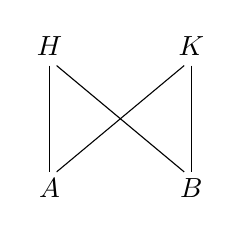
\begin{tikzpicture}[scale=0.9]
                \node [above] at (0,0) {$A$};
                \node [above] at (0,2) {$H$};
                \node [above] at (2,2) {$K$};
                \node [above] at (2,0) {$B$};
                \draw [-] (1.9,2) to (0.1,0.5);
                \draw [-] (2,2) to (2,0.5);
                \draw [-] (0,2) to (0,0.5);
                \draw [-] (0.1,2) to (1.9,0.5);
            \end{tikzpicture}
        \end{figure}
        But $A<H\cap K$, $B<H\cap K\Rightarrow A\vee B<H\cap K$. So $A\vee B\lhd H$, $A\vee B\lhd K$. That's contradictory! There is only one lower bound for $\{H,K\}$. Notice that $\{e\}<H\cap K$ so there exists at least one subgroup satisfies the condition. We have proved normality forms a lattice.
    \end{enumerate}
\end{answer}

$$ $$

\begin{ex}
    If $N_{1}\lhd G_{1}$, $N_{2}\lhd G_{2}$ then $(N_{1}\times N_{2})\lhd (G_{1}\times G_{2})$ and $(G_{1}\times G_{2})/(N_{1}\times N_{2})\cong (G_{1}/N_{1})\times(G_{2}/N_{2})$.
\end{ex}

\begin{answer}
    Take $a\in (N_{1}\times N_{2})$, $a=(n_{1},n_{2})$ where $n_{1}\in N_{1}$, $n_{2}\in N_{2}$. $\forall x\in (G_{1}\times G_{2})$, $x=(g_{1},g_{2})$ where $g_{1}\in G_{1}$, $g_{2}\in G_{2}$. $x^{-1}=(g_{1}^{-1},g_{2}^{-1})$, $x^{-1}ax=(g_{1}^{-1}n_{1}g_{1},g_{2}^{-1}n_{2}g_{2})$. $N_{1}\lhd G_{1}$, $N_{2}\lhd G_{2}$, so $g_{1}^{-1}n_{1}g_{1}\in N_{1}$, $g_{2}^{-1}n_{2}g_{2}\in N_{2}$. $x^{-1}ax\in (N_{1}\times N_{2})$. Thus $(N_{1}\times N_{2})\lhd (G_{1}\times G_{2})$.

    Assume $G_{1}=\bigcup\limits_{i\in I}N_{1}a_{i}$, $G_{2}=\bigcup\limits_{j\in J}N_{2}b_{j}$. Then $G_{1}\times G_{2}=\bigcup\limits_{i\in I}N_{1}a_{i}\times \bigcup\limits_{j\in J}N_{2}b_{j}$. Denote $A=\{a_{i}|i\in I\}$, $B=\{b_{j}|j\in J\}$. We construct two bijections $(G_{1}\times G_{2})/(N_{1}\times N_{2})\to A\times B$ and $(G_{1}/N_{1})\times(G_{2}/N_{2})$.\[f: N_{1}a_{i}\times N_{2}b_{j}\mapsto (a_{i},b_{j})\]\[g: (N_{1}a_{i}, N_{2}b_{j})\mapsto (a_{i},b_{j})\] Take $h=g^{-1}\circ f$, $f,g$ are bijections, so $h$ is an isomorphism. $(G_{1}\times G_{2})/(N_{1}\times N_{2})\cong (G_{1}/N_{1})\times(G_{2}/N_{2})$.
\end{answer}

$$ $$

\begin{ex}
    Let $N\lhd G$ and $K\lhd G$. If $N\cap K=\left\langle e\right\rangle$ and $N\vee K=G$, then $G/N\cong K$.
\end{ex}

\begin{answer}
    Assume $G=\bigcup\limits_{i\in I}Na_{i}$, we construct $f:k \to G /N$. We prove that $\forall x,y\in K$, $x,y$ belong to different cosets of $N$. Suppose not. $\exists x,y \in K$, $x,y\in Na_{i}$, then $xy^{-1}\in N\Rightarrow x=y$. That's contradictory! So $f$ is a monomorphism.

    $G=H\vee K$, so $G=HK$. we can write $x$ as $pq$, where $p\in H$, $q\in K$. $\left| G/H \right|=\left[G:H\right]=\left[HK:H\right]=\left[K:K\cap H\right]=\left| K \right| $. $f$ is a epimorphism.
    
    Thus, $G /N\cong K$.
\end{answer}

$$ $$

\begin{ex}
    If $f:G\to H$ is a homomorphism, $H$ is abelian and $N$ is a subgroup of $G$ containing $\mathrm{Ker}f$, then $N$ is normal in $G$.
\end{ex}

\begin{answer}
    Assume there exists $x\in G$, $x\notin N$ s.t. $f(x)\in f(N)$. $\exists n\in N$, $f(x)=f(n)$, $f(xn^{-1})=f(x)f(n)^{-1}=e'\Rightarrow xn^{-1}\in\mathrm{Ker}f\Rightarrow x\in N$. That's contradictory! $\forall x\in G$, $n\in N$, $f(x^{-1}nx)=f(x^{-1})f(n)f(x)=f(n)\in f(N)$, so $x^{-1}nx\in N$. Thus, $N\lhd G$.
\end{answer}

$$ $$

\begin{ex}
    \begin{enumerate}[(a)]
        \item Consider the subgroups $\left\langle 6\right\rangle$ and $\left\langle 30\right\rangle$ of $\mathbf{Z}$ and show that $\left\langle 6\right\rangle /\left\langle 30\right\rangle\cong Z_{5}$.
        \item For any $k,m>0$, $\left\langle k\right\rangle /\left\langle km\right\rangle\cong Z_{m}$; in particular, $\mathbf{Z}/\left\langle m\right\rangle=\left\langle 1\right\rangle /\left\langle m\right\rangle\cong Z_{m}$.
    \end{enumerate}
\end{ex}

\begin{answer}
    \begin{enumerate}[(a)]
        \item $\left\langle 6\right\rangle=\{6n|n\in \mathbf{Z}\}$, $\left\langle 30\right\rangle=\{30n|n\in \mathbf{Z}\}$. So $\left\langle 6\right\rangle/\left\langle 30\right\rangle=\{\left\langle 30\right\rangle, \left\langle 30\right\rangle +6, \left\langle 30\right\rangle +12, \left\langle 30\right\rangle +18, \left\langle 30\right\rangle +24\}\cong Z_{5}$
        \item $\left\langle km\right\rangle\lhd \left\langle k\right\rangle$, $\left\langle k\right\rangle=\bigcup\limits_{i\in I}(\left\langle km\right\rangle +a_{i})$. For $x\in \left\langle k\right\rangle$, $x\equiv a_{i}\mod km$, then $x\in \left\langle km \right\rangle +a_{i}$. $f:\left\langle k\right\rangle/\left\langle km\right\rangle\to \{a_{i}|i\in I\}$ defined by $f(\left\langle km\right\rangle +a_{i})=a_{i}$ is a bijection. We check that $g: \{a_{i}|i\in I\}\to Z_{m}$ is also a bijection. Define $b_{i}\equiv \frac{a_{i}}{k}\mod m$, $g(a_{i})=b_{i}$. If there exists $b_{i}=b_{j}$ for $i\neq j$, $a_{i}\equiv a_{j}\mod km$. That's contradictory! So $g$ is an injection. $g$ is obviously a surjection, so $g$ is a bijection. Take $h= g\circ f:\left\langle k\right\rangle /\left\langle km \right\rangle\to Z_{m}$ is a isomorphism, so $\left\langle k\right\rangle /\left\langle km \right\rangle\cong Z_{m}$.
    \end{enumerate}
\end{answer}

$$ $$

\begin{ex}
    If $f: G \to H$ is a homomorphism with kernel $N$ and $K<G$, then prove that $f^{-1}(f(K))=KN$. Hence $f^{-1}(f(K))=K$ if and only if $N<K$.
\end{ex}

\begin{answer}
    Take $x\in f^{-1}(f(K))$, then there exists $k\in K$ s.t. $f(x)=f(k)$. $f(xk^{-1})=f(x)f(k)^{-1}=e'\in f(K) \Rightarrow xk^{-1}\in\mathrm{Ker}f=N$. Thus, $x\in Nk\subset NK$, $f^{-1}(f(K))\subset NK$.

    $\forall x=nk\in NK$, where $n\in N$ and $k\in K$. $f(x)=f(n)f(k)=e'f(k)\in f(K)$, so $NK\subset f^{-1}(f(K))$.

    Thus, $f^{-1}(f(K))=NK$. Hence $f^{-1}(f(K))=K$ if and only if $N<K$.
\end{answer}

$$ $$

\begin{ex}
    If $N\lhd G$, $\left[G:H\right]$ finite, $H<G$, $\left| H \right| $ finite, and $\left[G:N\right]$ and $\left| H \right| $ are relatively prime, then $H<N$.
\end{ex}

\begin{answer}
    $N\lhd G\Rightarrow NH<G$. By the second isomorphism theorem, $NH /N\cong H/H\cap N\Rightarrow \left[NH:N\right]=\left[H:H\cap N\right]$. Assume $\left[G:N\right]=m$, $\left| H \right| =n$, $\left| G \right| =mnp$ where $(m,n)=1$. Then $\left| N \right| =np$, $N<NH$, assume $\left| NH \right| =knp$, $NH<G\Rightarrow knp|mnp\Rightarrow k|m$. $\left[NH:N\right]=\left[H:H\cap N\right]=k\Rightarrow k|n$. So $k=1$, $NH=N$ which means $H<N$.
\end{answer}

$$ $$

\begin{ex}
    If $N\lhd G$, $\left| N \right|$ finite, $H<G$, $\left[G:N\right] $ finite, and $\left[G:H\right]$ and $\left| N \right| $ are relatively prime, then $N<H$.
\end{ex}

\begin{answer}
    $N\lhd G\Rightarrow NH<G$. By the second isomorphism theorem, $NH /N\cong H/H\cap N\Rightarrow \left[NH:N\right]=\left[H:H\cap N\right]$. Assume $\left[G:H\right]=m$, $\left| N \right| =n$, $\left| G \right| =mnp$ where $(m,n)=1$. Then $\left| H \right| =np$, $H<NH$, assume $\left| NH \right| =knp$, $NH<G\Rightarrow knp|mnp\Rightarrow k|m$. $\left[NH:N\right]=\left[H:H\cap N\right]=kp\Rightarrow kp|np\Rightarrow k|n$. So $k=1$, $NH=H$ which means $N<H$.
\end{answer}

$$ $$

\begin{ex}
    If $H$ is a subgroup of $Z(p^{\infty})$ and $H\neq Z(p^{\infty})$, then $Z(p^{\infty}) /H\cong Z(p^{\infty})$.
\end{ex}

\begin{answer}
    From \textbf{Exercise 1.3.7}(b), we know that $H$ has the form $\left\langle \bar{\frac{1}{p^{n}}}\right\rangle$. Take $x_{i}=\bar{\frac{1}{p^{n+i}}}+H$, $x_{1}=\bar{\frac{1}{p^{n+1}}}+H$. \[\sum_{m=1}^{p}x_{1}=\bar{\frac{p}{p^{n+1}}}+pH=\bar{\frac{1}{p^{n}}}+H=H\] \[\sum_{m=1}^{p}x_{i}=\bar{\frac{p}{p^{n+i}}}+pH=\bar{\frac{1}{p^{n+i-1}}}+H=x_{i-1}\] Take $A=\{x_{i}|i\in \mathbf{Z}_{+}\}$, $\left\langle A\right\rangle\cong Z(p^{\infty})$ by \textbf{Exercise 1.3.7}(e). $\forall x\in \left\langle A\right\rangle$, $x\in Z(p^{\infty}) /H$, so $\left\langle A\right\rangle\subset Z(p^{\infty}) /H$. Take $x\in Z(p^{\infty}) /H$, $x=y+H$ where $y=\sum\limits_{i=1}^{m}\frac{a_{i}}{p^{n+i}}$, $x=\sum\limits_{i=1}^{m}(\frac{a_{i}}{p^{n+i}}+H)\in \left\langle A\right\rangle$. Thus, $Z(p^{\infty}) /H\subset \left\langle A\right\rangle$, $\left\langle A\right\rangle=Z(p^{\infty}) /H\cong Z(p^{\infty})$.
\end{answer}
\section{Symmetric, alternating, and dihedral groups}
\begin{ex}
    Find four different subgroups of $S_{4}$ that are isomorphic to $S_{3}$ and nine isomorphic to $S_{2}$.
\end{ex}

\begin{answer}
    $S_{4}=\{(1), (12), (13), (14), (23), (24), (34), (123), (124), (132),\\ (142), (134), (143), (234), (243), (12)(34), (13)(24), (14)(23), (1234),\\ (1243), (1324), (1342), (1423), (1432)\}$.

    $A_{1}=\{(1), (12), (13), (23), (123), (132)\}$;

    $A_{2}=\{(1), (12), (14), (24), (124), (142)\}$;

    $A_{3}=\{(1), (13), (14), (34), (134), (143)\}$;

    $A_{4}=\{(1), (23), (24), (34), (234), (243)\}$;
    
    $A_{1}\cong A_{2}\cong A_{3}\cong A_{4}$.

    $B_{1}=\{(1), (12)\}$; $B_{2}=\{(1),(13)\}$; $B_{3}=\{(1),(14)\}$; $B_{4}=\{(1), (23)\}$; $B_{5}=\{(1),(24)\}$; $B_{6}=\{(1), (34)\}$; $B_{7}=\{(1),(12)(34)\}$; $B_{8}=\{(1),(13)(24)\}$; $B_{9}=\{(14)(23)\}$;

    $B_{1}\cong B_{2}\cong B_{3}\cong B_{4}\cong B_{5}\cong B_{6}\cong B_{7}\cong B_{8}\cong B_{9}$.
\end{answer}

$$ $$

\begin{ex}
    \begin{enumerate}[(a)]
        \item $S_{n}$ is generated by the $n-1$ transpositions $(12)$, $(13)$, $(14)$, $\dots$, $(1n)$.
        \item $S_{n}$ is generated by the $n-1$ transpositions $(12), (23), (34),\dots, (n-1\, n)$.
    \end{enumerate}
\end{ex}

\begin{answer}
    \begin{enumerate}[(a)]
        \item $\forall x\in S_{n}$, $x$ can be written as a product of transpositions. Actually, for any transposition $(ij)$, we can obtain it by $(1i)(1j)(1i)=(ij)$. So $x\in \left\langle (12), (13),\dots,(1n)\right\rangle$, $S_{n}\subset\left\langle(12), (13),\dots,(1n)\right\rangle$.
        \item We can contruct $(1i)$ inductively since $(1i)=(1\, i-1)(i-1\, i)(1\, i-1)$. From (a), we have $\forall x\in S_{n}$, $x\in \left\langle (12), (13),\dots,(1n)\right\rangle$. Thus $S_{n}\subset\left\langle(12), (13),\dots,(1n)\right\rangle\subset \left\langle (12), (23), (34),\dots, (n-1\, n)\right\rangle$.
    \end{enumerate}
\end{answer}

$$ $$

\begin{ex}
    If $\sigma=(i_{1}i_{2}\cdots i_{r})\in S_{n}$ and $\tau\in S_{n}$, then $\tau\sigma\tau^{-1}$ is the $r$-cycle $(\tau(i_{1})\tau(i_{2})\cdots\tau(i_{r}))$.
\end{ex}

\begin{answer}
    $\sigma(i_{n})=i_{n+1}$ for $n=1,2,\dots,r-1$, $\sigma(i_{r})=i_{1}$. Assume $\tau(i_{n})=j_{n}$, $n=1,2,\dots,r-1$ and $I=\{i_{n}|n=1,2,\dots,r-1\}$, $J=\{j_{n}|n=1,2,\dots,r-1\}$. For $x\notin J$, $\tau\sigma\tau^{-1}(x)=\tau\tau^{-1}(x)=x$. For $x=j_{k}\in J$, $\tau^{-1}(x)=i_{k}$, $\sigma(\tau^{-1}(x))=i_{k+1}$, $\tau(\sigma(\tau^{-1}(x)))=j_{k+1}$ and $\tau\sigma\tau^{-1}(j_{r})=j_{1}$. Thus $\tau\sigma\tau^{-1}=(\tau(i_{1})\tau(i_{2})\cdots\tau(i_{r}))$.
\end{answer}

$$ $$

\begin{ex}
    \begin{enumerate}[(a)]
    \item $S_{n}$  is generated by $\sigma_{1}=(12)$ and $\tau=(123\cdots n)$.
    \item $S_{n}$ is generated by $(12)$ and $(23\cdots n)$.
    \end{enumerate}
\end{ex}

\begin{answer}
    \begin{enumerate}[(a)]
        \item Denote $\sigma_{i}=\tau\sigma_{i-1}\tau^{-1}$. Applying \textbf{Exercise 1.6.3}, $\sigma_{i}=(i\, i+1)$. By \textbf{Exercise 1.6.2}(b), $S_{n}\subset\left\langle (12), (23), (34),\dots, (n-1\, n)\right\rangle=\left\langle\sigma_{1}, \sigma_{2},\dots,\sigma_{n-1}\right\rangle\subset \left\langle \tau, \sigma_{1}\right\rangle$. $S_{n}$ can be generated by $\tau$ and $\sigma_{1}$.
        \item Denote $\sigma_{1}=(12)$, $\tau=(23\cdots n)$, $\sigma_{i}=\tau\sigma_{i-1}\tau^{-1}$. Applying \textbf{Exercise 1.6.3},$\sigma_{i}=(1\, i+1)$. By \textbf{Exercise 1.6.2}(a), $S_{n}\subset\left\langle(12), (13),\dots,(1n)\right\rangle=\left\langle \sigma_{1},\sigma_{2},\dots,\sigma_{n-1}\right\rangle\subset\left\langle \tau,\sigma_{1}\right\rangle$. $S_{n}$ can be generated by $\tau$ and $\sigma_{1}$.
    \end{enumerate}
\end{answer}

$$ $$

\begin{ex}
    Let $\sigma, \tau \in S_{n}$. If $\sigma$ is even (odd), then so is $\tau\sigma\tau^{-1}$.
\end{ex}

\begin{answer}
    Assume $\sigma=(x_{1}x_{2})\cdots(x_{2n-1}x_{2n})$, $\tau=(y_{1}y_{2})\cdots(y_{2m-1}y_{2m})$. Then $\tau^{-1}=(y_{2m-1}y_{2m})\cdots(y_{1}y_{2})$. $\sigma$ is odd (even) if an only if $n$ is odd (even). $\tau\sigma\tau^{-1}$ has $2m+n$ transpositions. We can add $(ij)=(ji)=(1)$ into some segments of $\tau\sigma\tau^{-1}$ without changing it. So $\tau\sigma\tau^{-1}$ is odd (even) if and only if $2m+n$ is odd (even). $2m+n\equiv n\mod 2$ so $\tau\sigma\tau^{-1}$ is odd (even) if and only if $\sigma$ is odd (even).
\end{answer}

$$ $$

\begin{ex}
    $A_{n}$ is the only subgroup of $S_{n}$ of index 2.
\end{ex}

\begin{answer}
    For any subgroup $N<S_{n}$ and $\left[S_{n}:N\right]=2$, we have $N\lhd S_{n}$.

    Assume there exists $k$-circle $\sigma=(i_{1}i_{2}\cdots i_{k})\in N$. Then for any other $k$-circle $(j_{1}j_{2}\cdots j_{k})$, take $\tau=(i_{i}j_{1})(i_{2}j_{2})\cdots(i_{k}j_{k})$, by \textbf{Exercise 1.6.3}, $\tau\sigma\tau^{-1}=(j_{1}j_{2}\cdots j_{k})\in N$. Thus $N$ contains all the $k$-circles.

    For $n\geq 5$. If there exists 3-circle in $N$, then all the 3-circles are contained in $N$, $A_{n}\subset N\subset S_{n}\Rightarrow A_{n}=N$.

    If there exists 2-circle in $N$, then all the 2-circles are contained in $N$. Notice $(1i)(1j)=(1ij)\in N$ is a 3-circle, so $A_{n}=N$.

    If there only contain $x$ in the form of $(a_{i}a_{2}\cdots a_{n_{1}})(b_{1}b_{2}\cdots b_{n_{2}})\cdots$ where $n_{i}\geq 4$ and every two circles are disjoint. Take $\tau_{i}:\{a_{i}|i=1,2,\dots,n_{1}\}\to \{a_{i}|i=1,2,\dots,n_{1}\}$. We can obtain product of two $n_{1}$-circles\[x^{-1}\tau x \tau^{-1}=(a_{1}a_{2}\cdots a_{n_{1}})(\tau(a_{1})\tau(a_{2})\cdots \tau(a_{n}))\in N\] By the arbitrariness of $\tau$, take \[(\tau(a_{1})\tau(a_{2})\cdots \tau(a_{n}))=(a_{1}a_{4}a_{5}\cdots a_{n}a_{3}a_{2})\] then $x^{-1}\tau x \tau^{-1}=(a_{1}a_{3})(a_{2}a_{4})$ is a product of 2-circles. We can take $a_{1}, a_{2}, a_{3}, a_{4}$ arbitrarily. WLOG, take $(12)(34)\in N$ and $(12)(35)\in N$, $(12)(35)(12)(34)=(345)\in N$. Then there exists 3-circle in $N$, $N=A_{n}$.

    In conlusion, when $n\geq 5$, $S_{n}$ has only one normal subgroup $A_{n}$.

    For $n=2,3,4$, we can verify it by enumeration.
\end{answer}

$$ $$

\begin{ex}
    Show that $N=\{(1),(12)(34),(13)(24),(14)(23)\}$ is a normal subgroup of $S_{4}$ contained in $A_{4}$ such that $S_{4} /N\cong S_{3}$ and $A_{4} /N\cong Z_{3}$.
\end{ex}

\begin{answer}
    Assume $\sigma=(i_{1}i_{2})(i_{3}i_{4})\in N$, $\forall \tau\in S_{4}$, $\tau(i_{n})=j_{n}$, $J=\{j_{n}|n=1,2,3,4\}$. For $x\notin J$, $\tau\sigma\tau^{-1}(x)=\tau\tau^{-1}(x)=x$. For $x=j_{k}\in J$, $\tau^{-1}(x)=i_{k}$, $\sigma\tau^{-1}(x)=i_{3k-4\left[\frac{k}{2}\right]-1}$, $\tau\sigma\tau^{-1}(x)=(\tau(i_{i})\tau(i_{2}))(\tau(i_{3})\tau(i_{4}))\in N$. So $N\lhd S_{4}$. $S_{4} /N=\{N, N(12), N(13), N(23), N(123), N(132)\}\cong S_{3}$. $A_{4} /N=\{N, N(123), N(132)\}\cong Z_{3}$.
\end{answer}

$$ $$

\begin{ex}
    The group $A_{4}$ has no subgroup of order $6$.
\end{ex}

\begin{answer}
    $\left| A_{4} \right| =12$, assume there exists $N<A_{4}$, $\left| N \right| =6$. Then $N\lhd A_{4}$. From \textbf{Exercise 1.6.6}, we know that all 3-circles are contained in $N$. But there're 8 3-circles in total, so $N$ can't exist.
\end{answer}

$$ $$

\begin{ex}
    For $n\geq 3$ let $G_{n}$ be the multiplicaive group of complex matrices generated by $x=\begin{pmatrix}
        0&1\\1&0
    \end{pmatrix}$ and $y=\begin{pmatrix}
        e^{2\pi i/n}&0\\0&e^{-2\pi i/n}
    \end{pmatrix}$, where $i^{2}=-1$. Show that $G_{n}\cong D_{n}$.
\end{ex}

\begin{answer}
    Take a mapping $f:G_{n}\to D_{n}$ as $f(x)=(2\,n)(3\,n-1)\cdots$, $f(y)=(123\cdots n)$. $\left| f(x) \right|=\left| x \right| =2$, $\left| f(y) \right| =\left| y \right| =n$. $f$ is obviously a monomorphism. $\forall a\in D_{n}$, $a=f(x)^{n}f(y)^{m}, m=1,2$, then $a=f(x^{n}y^{m})$, $f$ is a epimorphism. Thus $G_{n}\cong D_{n}$. 
\end{answer}

$$ $$

\begin{ex}
    Let $a$ be the generator of order $n$ of $D_{n}$. Show that $\left\langle a\right\rangle\lhd D_{n}$ and $D_{n} /\left\langle a\right\rangle\cong Z_{2}$.
\end{ex}

\begin{answer}
    $\left| \left\langle a\right\rangle \right| =n$, $b$ is the other generator of $D_{n}$, $a^{n}=b^{2}=(1)$. $\forall k\in \mathbf{Z}$, $a^{k}b=ba^{-k}$ can be easily proved by induction. So $\forall x=a^{m}b^{n}\in D_{n}$, $x=a^{m'}b^{n'}$, here $m'\equiv m\mod 2$, $n'\equiv n\mod 2$. $D_{n}=\{e, a, a^{2}, \dots, a^{n-1}, b, ba, \\\dots, ba^{n-1}\}$. $\left| D_{n} \right| =2n$. Thus, $\left\langle a\right\rangle\lhd D_{n}$. $D_{n} /\left\langle a\right\rangle=\{\left\langle a\right\rangle, \left\langle a\right\rangle b\}\cong Z_{2}$.
\end{answer}

$$ $$

\begin{ex}
    Find all normal subgroups of $D_{n}$.
\end{ex}

\begin{answer}
    The subgroups of $\left\langle a\right\rangle$ is always normal in $D_{n}$. $\left\langle a^{m}\right\rangle <\left\langle a\right\rangle$. $\forall x\in D_{n}$ and $a^{km}\in \left\langle a^{m}\right\rangle$, $x=a^{t}$ or $x=ba^{t}$. \[x^{-1}a^{km}x=a^{-t}a^{km}a^{t}=a^{km}\in\left\langle a^{m}\right\rangle\] or \[x^{-1}a^{km}x=a^{-t}b^{-1}a^{km}ba^{t}=a^{-t}ba^{km}ba^{t}=a^{-t}a^{-km}b^{2}a^{t}=a^{-km}\in \left\langle a^{m}\right\rangle\] so $\left\langle a^{m}\right\rangle \lhd D_{n}$.

    Consider the subgroup $S$ which only contains $ba^{i}, i=1,\dots, n$. Since $ba^{i}\cdot ba^{j}=a^{j-i}\in S\,(i\neq j)$, so $S=\{e, ba^{k}\}$.

    If $n$ is odd, take $x=a^{\frac{n-1}{2}}\in D_{n}$. \[x^{-1}ba^{k}x=a^{\frac{1-n}{2}}ba^{k}a^{\frac{n-1}{2}}=ba^{k+n-1}\notin S\] so $S\ntriangleleft D_{n}$ for all $k=1,2,\dots,n$.

    If $n$ is even, take $x=a^{\frac{n-2}{2}}\in D_{n}$, $n\geq 6$. \[x^{-1}ba^{k}x=a^{\frac{2-n}{2}}ba^{k}a^{\frac{n-2}{2}}=ba^{k+n-2}\notin S\] so $S\ntriangleleft D_{n}$ for all $k=1,2,\dots,n$.

     If $n=2$, all the subgroups are normal since $\left| D_{2} \right| =4$.

     For subgroup $S$ contains both $ba^{i}$ and $a^{j}$. It can be written as $S=\left\langle a^{d}, ba^{r}\right\rangle$, where $d|n$, $0\leq r\leq d-1$. If $\exists a^{m}, a^{n}\in S$, $(m,n)=d$, then there exist $x,y\in \mathbf{Z}$ s.t. $a^{mx+ny}=a^{d}\in \mathbf{Z}$. Thus, $S=\left\langle a^{d},ba^{r}\right\rangle$.

     Take $x=a^{\frac{n-w}{2}}$, then $x^{-1}ba^{r}x=ba^{r+n-w}$.
     
     If $d\geq 3$, take $w\equiv n\mod 2$, $x^{-1}ba^{r}x\notin S$.

     If $d=2$, then $n=2s$ and $S=\{e, a^{s}, ba^{s}, b\}$. $Sa^{k}=\{a^{k}, a^{s+k},ba^{s-k}, ba^{-k}\}$, $k=1,2,\dots, s-1$. $ba^{k}=ba^{-k}$ or $ba^{k}=ba^{s-k}\Rightarrow k=\frac{s}{2}$. So for $s=2$, $n=4$, $S$ is a normal subgroup of $D_{4}$.
\end{answer}

$$ $$

\begin{ex}
    The center of the group $D_{n}$ is $\left\langle e\right\rangle$ if $n$ is odd and isomorphic to $Z_{2}$ if $n$ is even.
\end{ex}

\begin{answer}
    If $n$ is odd, $C$ is the center of $D_{n}$, $C\lhd D_{n}\Rightarrow C<\left\langle a\right\rangle$. Take $a^{d}\in C$, $x=ba^{m}$, \[x^{-1}ax=a^{-m}b^{-1}a^{d}ba^{m}=a^{-m}ba^{d}ba^{m}=a^{-d}=a^{d}\] so $d=0$, $C=\{e\}$.

    If $n$ is even, $n\geq 6$. $C$ is the center of $D_{n}$. $C\lhd D_{n}\Rightarrow C<\left\langle a\right\rangle$ or $C=\{e,ba^{k}\}$.
    
    If $C=\{e,ba^{k}\}$, $C\cong Z_{2}$.
    
    If $C<\left\langle a\right\rangle$,take $a^{d}\in C$, $x=ba^{m}$, \[x^{-1}ax=a^{-m}b^{-1}a^{d}ba^{m}=a^{-m}ba^{d}ba^{m}=a^{-d}=a^{d}\] so $d=\frac{n}{2}$ or $d=0$, $C=\{a^{\frac{n}{2}},e\}\cong Z_{2}$.
\end{answer}

$$ $$

\begin{ex}
    For each $n\geq 3$ let $P_{n}$ be a regular polygon of $n$ sides (for $n=3$, $P_{n}$ is an equilateral triangle; for $n=4$, a square). A \emph{symmetry} of $P_{n}$ is a bijection $P_{n}\to P_{n}$ that preserves distances and maps adjacent vertices on to adjacent vertices.
    
    \begin{enumerate}[(a)]
        \item The set $D_{n}^{*}$ of all symmetries of $P_{n}$ is a group under the binary operation of composition of functions.
        \item Every $f\in D_{n}^{*}$ is completely determined by its actions on the vertices of $P_{n}$. Number the vertices consecutively $1,2,\dots, n$; then each $f\in D_{n}^{*}$ determines a unique permutation $\sigma_{f}$ of $\{1,2,\dots, n\}$. The assignment $f\mapsto \sigma_{f}$ defines a monomorphism of groups $\varphi:D_{n}^{*}\to S_{n}$.
        \item $D_{n}^{*}$ is generated by $f$ and $g$, where $f$ is a rotation of $2\pi /n$ degrees about the center of $P_{n}$ and $g$ is a reflection about the ``diameter'' through the center and vertex 1.
        \item $\sigma_{f}=(123\cdots n)$ and $\sigma_{g}=\begin{pmatrix}
            1&2&3&\cdots&n-1&n\\1&n&n-1&\cdots&3&2
        \end{pmatrix}$, whence \\$\mathrm{Im}\varphi=D_{n}$ and $D_{n}^{*}\cong D_{n}$.
    \end{enumerate}
\end{ex}

\begin{answer}
    In the following analysis, all the numbers are $\mod n$.
    \begin{enumerate}[(a)]
        \item Consider $n$ points $A_{i}=(\cos \frac{2\pi i}{n},\sin \frac{2\pi i}{n})^{t}$, $i=1,2,\dots,n$. $f$ is the transposition of $A_{i}\mapsto A_{j}$ with the consevation of $n$ regular polygon structure. So $f$ must be a bijection. $D_{n}^{*}$ is the set of $f$. By the definition, $D_{n}^{*}\subset S_{n}$. We prove $D_{n}^{*}$ is ta subgroup of $S_{n}$.
        
        Notice that $A_{i+1}=\begin{pmatrix}
            \cos \frac{2\pi i}{n}&-\sin\frac{2\pi i}{n}\\\sin\frac{2\pi i}{n}&\cos \frac{2\pi i}{n}
        \end{pmatrix}A_{i}$.
        
        Denote $X=\begin{pmatrix}
            \cos \frac{2\pi i}{n}&-\sin\frac{2\pi i}{n}\\\sin\frac{2\pi i}{n}&\cos \frac{2\pi i}{n}
        \end{pmatrix}$. To construct the polygon,  we must have \[f(A_{i+1})=\begin{pmatrix}
            \cos \frac{2\pi i}{n}&-\sin\frac{2\pi i}{n}\\\sin\frac{2\pi i}{n}&\cos \frac{2\pi i}{n}
        \end{pmatrix}f(A_{i})\] or \[f(A_{i})=\begin{pmatrix}
            \cos \frac{2\pi i}{n}&-\sin\frac{2\pi i}{n}\\\sin\frac{2\pi i}{n}&\cos \frac{2\pi i}{n}
        \end{pmatrix}f(A_{i+1})\] We need to verify that $\forall f_{1}, f_{2}\in D_{n}^{*}$, $f_{1}f_{2}^{-1}\in D_{n}^{*}$. Assume $B_{i}=f_{2}(A_{i})$, $B_{i+1}=f_{2}(A_{i+1})$. Then $B_{i}=XB_{i+1}$ or $B_{i}=X^{-1}B_{i+1}$. Denote $B_{i}=A_{j}$, then $B_{i+1}=A_{j-1}$ or $B_{i+1}=A_{j+1}$. WLOG, assume $B_{i+1}=A_{j+1}$, then $f_{1}(A_{j})=Xf_{1}(A_{j+1})$ or $f_{1}(A_{j})=X^{-1}f_{1}(A_{j-1})$. So $f_{1}f_{2}^{-1}\in D_{n}^{*}$. $D_{n}^{*}$ is a subgroup of $S_{n}$.
        \item Assume $A_{i}=f(A_{1})$. If $f(A_{2})=A_{i+1}$, since $f$ is a bijection, by induction, we can prove $f(A_{k})=A_{k+i-1}$. $\varphi: D_{n}^{*}\to S_{n}$ can be defined as $\varphi: f\mapsto (1i\,2i-1\,3i-2\cdots)$. If $f(A_{2})=A_{i-1}$, similarly, we can also prove $f(A_{k})=A_{i+1-k}$. $\varphi$ can be defined as $\varphi: f\mapsto (1i)(2\,i-1)(3\,i-2)\cdots$. This means $f$ is completely determined by $f(A_{1})$ and $f(A_{2})$. $D_{n}^{*}$ can be embedded into $S_{n}$.
        \item Denote $\alpha=\begin{pmatrix}
            \cos \frac{2\pi i}{n}&-\sin\frac{2\pi i}{n}\\\sin\frac{2\pi i}{n}&\cos \frac{2\pi i}{n}
        \end{pmatrix}$, $\beta=\begin{pmatrix}
            1&0\\0&1
        \end{pmatrix}$. $f:A_{i}\mapsto \alpha A_{i}$, $g:A_{i}\mapsto \beta A_{i}$. $f$ is the rotation of $\frac{2\pi}{n}$ degrees counter-clockwisely. $g$ is the reflection about $x$-axis. Now we prove $\forall x\in D_{n}^{*}$, $x$ can be factorised into finite product of $f$ and $g$. From (b), $x$ is fully defined by $x(A_{1})$ and $x(A_{2})$. Assume $x(A_{1})=A_{i}$.

        If $x(A_{2})=A_{i+1}$, $x(A_{k})=A_{i-1+k}=\alpha^{i-1}A_{k}$, $k=1,2,\dots,n$. So $x=f^{i-1}$.

        If $x(A_{2})=A_{i-2}$, $x(A_{k})=A_{i+1-k}=\alpha^{i+1}A_{-k}=\alpha^{i+1}\beta A_{k}$. So $x=f^{i+1}g$. Thus $D_{4}^{*}\subset\left\langle f,g\right\rangle$.
        \item $\alpha^{n}=\beta^{2}=\begin{pmatrix}
            1&0\\0&1
        \end{pmatrix}$. We can easily verify that $\left| f \right| =n$ and $\left| g \right| =2$. From \textbf{Exercise 1.6.9}, $\left\langle f,g\right\rangle\cong D_{n}$, $\left| \left\langle f,g\right\rangle \right| =\left| D_{n} \right| =2n$. From (b), $x\in D_{n}^{*}$ if completely determined by $x(A_{1})$ and $x(A_{2})$. There are $2n$ different ways to obtain $x(A_{1})$ and $x(A_{2})$. So $\left| D_{n}^{*} \right| =\left| \left\langle f,g\right\rangle \right| =2n$. $D_{n}^{*}\subset \left\langle f,g\right\rangle$, so $D_{n}^{*}=\left\langle f,g\right\rangle$. Thus, $D_{n}^{*}\cong \left\langle f,g\right\rangle\cong D_{n}$.
    \end{enumerate}
\end{answer}
\section{Categories: products, coproducts, and free objects}
\begin{ex}
    A \emph{pointed set} is a pair $(S,x)$ with $S$ a set and $x\in S$. A morphism of pointed sets $(S,x)\to (S', x')$ is a triple $(f,x,x')$, where $S\to S'$ is a function such that $f(x)=x'$. Show that pointed sets form a category.
\end{ex}

\begin{answer}
    Let $\mathcal{S}$ be the category and 4 objects of $\mathcal{S}$ are $(A,a)$, $(B,b)$, $(C,c)$, $(D,d)$. $f$, $g$ and $h$ are morphisms defined by $f:A\to B$, $g:B\to C$, $h:C\to D$ with $f(a)=b$, $g(b)=c$, $h(c)=d$.

    \begin{figure}[H]\centering
        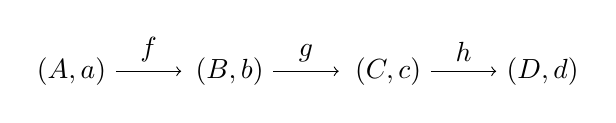
\begin{tikzpicture}
            \node [left] at (0,1) {$(A,a)$};
            \node [left] at (2,1) {$(B,b)$};
            \node [left] at (4,1) {$(C,c)$};
            \node [left] at (6,1) {$(D,d)$};
            \draw [->] (0,1)-- node [above, pos=0.5]{$f$}(0.83,1);
            \draw [->] (2,1)-- node [above, pos=0.5]{$g$}(2.83,1);
            \draw [->] (4,1)-- node [above, pos=0.5]{$h$}(4.83,1);
        \end{tikzpicture}
        \caption*{category $\mathcal{S}$}
    \end{figure}
    \[\mathrm{hom}(A,B)\times\mathrm{hom}(B,C)\to \mathrm{hom}(A,C)\]because $g\circ f:A\to C$ with $g(f(a))=g(b)=c=g\circ f(a)$. Similarly, $(h\circ g)\circ f=h\circ (g\circ f)$ with $(h\circ g)\circ f(a)=h\circ (g\circ f)(a)=d$. Take $1_{B}$ consist of those functions $i:B\to B$ with $i(b)=b$. Then $1_{B}\circ f=f$ and $g\circ 1_{B}=g$. So $\mathcal{S}$ is a category.
\end{answer}

$$ $$

\begin{ex}
    If $f:A\to B$ is an equivalence in a category $\mathcal{C}$ and $g:B\to A$ is the morphism such that $g\circ f=1_{A}$, $f\circ g=1_{B}$, show that $g$ is unique.
\end{ex}

\begin{answer}
    Assume there exist $g$ and $g'$ satisfies the condition.

    \begin{figure}[H]\centering
        \subfigure{
            \begin{minipage}[c]{0.3\linewidth}
                \centering
                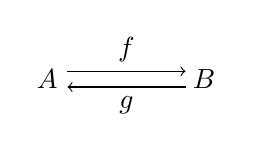
\begin{tikzpicture}
                    \node [left] at (0,1) {$A$};
                    \node [left] at (2,1) {$B$};
                    \draw [->] (0,1.1)-- node [above, pos=0.5]{$f$} (1.5,1.1);
                    \draw [<-] (0,0.9)-- node [below, pos=0.5]{$g$} (1.5,0.9);
                \end{tikzpicture}
            \end{minipage}
        }
        \subfigure{
            \begin{minipage}[c]{0.3\linewidth}
                \centering
                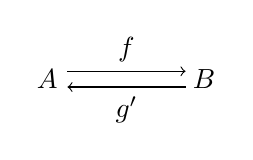
\begin{tikzpicture}
                    \node [left] at (0,1) {$A$};
                    \node [left] at (2,1) {$B$};
                    \draw [->] (0,1.1)-- node [above, pos=0.5]{$f$} (1.5,1.1);
                    \draw [<-] (0,0.9)-- node [below, pos=0.5]{$g'$} (1.5,0.9);
                \end{tikzpicture}
            \end{minipage}
        }
    \end{figure}
    So $g'\circ(f\circ g)=g'\circ 1_{B}=g'=(g'\circ f)\circ g=1_{A}\circ g =g$.
\end{answer}

$$ $$

\begin{ex}
    In the category $\mathcal{G}$ of groups, show that the group $G_{1}\times G_{2}$ together with the homomorphisms $\pi_{1}:G_{1}\times G_{2}\to G_{1}$ and $\pi_{2}:G_{1}\times G_{2}\to G_{2}$ is a product for $\{G_{1},G_{2}\}$.
\end{ex}

\begin{answer}
    Take $\tau_{1}:G_{1}\to G_{1}\times G_{2}$ as $\tau_{1}(g_{1})=(g_{1},e)$; $\tau_{2}:G_{2}\to G_{1}\times G_{2}$ as $\tau_{2}(g_{2})=(e,g_{2})$; $\pi_{1}:G_{1}\times G_{2}\to G_{1}$ as $\pi_{1}(g_{1},g_{2})=g_{1}$; $\pi_{2}:G_{1}\times G_{2}\to G_{2}$ as $\pi_{2}(g_{1},g_{2})=g_{2}$. Then

    \begin{figure}[H]\centering
        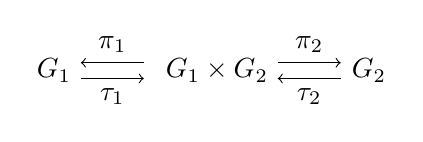
\begin{tikzpicture}
            \node [left] at (0,1) {$G_{1}$};
            \node [left] at (2.5,1) {$G_{1}\times G_{2}$};
            \node [left] at (4,1) {$G_{2}$};
            \draw [<-] (0,1.1)-- node [above, pos=0.5]{$\pi_{1}$} (0.8,1.1);
            \draw [->] (0,0.9)-- node [below, pos=0.5]{$\tau_{1}$} (0.8,0.9);
            \draw [->] (2.5,1.1)-- node [above, pos=0.5]{$\pi_{2}$} (3.3,1.1);
            \draw [<-] (2.5,0.9)-- node [below, pos=0.5]{$\tau_{2}$} (3.3,0.9);
        \end{tikzpicture}
    \end{figure}
    For any object $B$ such that

    \begin{figure}[H]\centering
        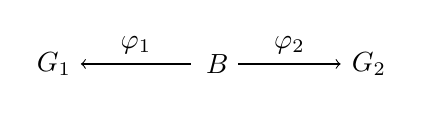
\begin{tikzpicture}
            \node [left] at (0,1) {$G_{1}$};
            \node [left] at (2,1) {$B$};
            \node [left] at (4,1) {$G_{2}$};
            \draw [<-] (0,1)-- node [above, pos=0.5]{$\varphi_{1}$} (1.4,1);
            \draw [->] (2,1)-- node [above, pos=0.5]{$\varphi_{2}$} (3.3,1);
        \end{tikzpicture}
    \end{figure}
    For any $x\in B$, define $f:B\to G_{1}\times G_{2}$ as $f(x)=(\varphi_{1}(x), \varphi_{2}(x))$. Then $\pi_{1}(f(x))=\varphi_{1}(x)$, $\pi_{1}\circ f=\varphi_{1}$, $\pi_{2}(f(x))=\varphi_{2}(x)$, $\pi_{2}\circ f=\varphi_{2}$. Thus
    
    \begin{figure}[H]\centering
        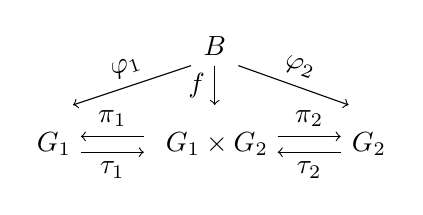
\begin{tikzpicture}
            \node [left] at (0,1) {$G_{1}$};
            \node [left] at (2.5,1) {$G_{1}\times G_{2}$};
            \node [left] at (4,1) {$G_{2}$};
            \draw [<-] (0,1.1)-- node [above, pos=0.5]{$\pi_{1}$} (0.8,1.1);
            \draw [->] (0,0.9)-- node [below, pos=0.5]{$\tau_{1}$} (0.8,0.9);
            \draw [->] (2.5,1.1)-- node [above, pos=0.5]{$\pi_{2}$} (3.3,1.1);
            \draw [<-] (2.5,0.9)-- node [below, pos=0.5]{$\tau_{2}$} (3.3,0.9);
            \node [above] at (1.7,2) {$B$};
            \draw [->] (1.7,2)-- node [left, pos=0.5]{$f$} (1.7,1.5);
            \draw [->] (1.4,2)-- node [above, pos=0.5, sloped]{$\varphi_{1}$} (-0.1,1.5);
            \draw [->] (2,2)-- node [above, pos=0.5, sloped]{$\varphi_{2}$} (3.4,1.5);
        \end{tikzpicture}
    \end{figure}
    Next we verify the uniqueness. If there exist $f$ and $f'$ satisfies the condition, \[\pi_{1}(f(x))=\pi_{1}(f'(x))=\varphi_{1}(x)\]\[\pi_{2}(f(x))=\pi_{2}(f'(x))=\varphi_{2}(x)\]Thus $f(x)=f'(x)$ for all $x\in B$, so $f=f'$.
\end{answer}

$$ $$

\begin{ex}
    In the category $\mathcal{A}$ of abelian groups, show that the group $A_{1}\times A_{2}$ together with the morphisms $\tau_{1}:A_{1}\to A_{1}\times A_{2}$ and $\tau_{2}:A_{2}\to A_{1}\times A_{2}$ is a coproduct of $\{A_{1}, A_{2}\}$.
\end{ex}

\begin{answer}
    Take $\tau_{1}:A_{1}\to A_{1}\times A_{2}$ as $\tau_{1}(a_{1})=(a_{1},e)$; $\tau_{2}:A_{2}\to A_{1}\times A_{2}$ as $\tau_{2}(a_{2})=(e,a_{2})$; $\pi_{1}:A_{1}\times A_{2}\to A_{1}$ as $\pi_{1}(a_{1},a_{2})=a_{1}$; $\pi_{2}:A_{1}\times A_{2}\to A_{2}$ as $\pi_{2}(a_{1},a_{2})=a_{2}$. Then

    \begin{figure}[H]\centering
        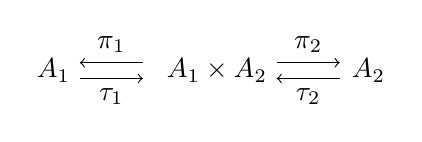
\begin{tikzpicture}
            \node [left] at (0,1) {$A_{1}$};
            \node [left] at (2.5,1) {$A_{1}\times A_{2}$};
            \node [left] at (4,1) {$A_{2}$};
            \draw [<-] (0,1.1)-- node [above, pos=0.5]{$\pi_{1}$} (0.8,1.1);
            \draw [->] (0,0.9)-- node [below, pos=0.5]{$\tau_{1}$} (0.8,0.9);
            \draw [->] (2.5,1.1)-- node [above, pos=0.5]{$\pi_{2}$} (3.3,1.1);
            \draw [<-] (2.5,0.9)-- node [below, pos=0.5]{$\tau_{2}$} (3.3,0.9);
        \end{tikzpicture}
    \end{figure}
    For any object $B$ such that

    \begin{figure}[H]\centering
        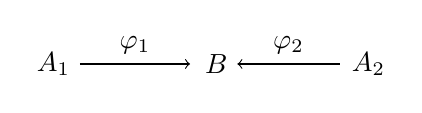
\begin{tikzpicture}
            \node [left] at (0,1) {$A_{1}$};
            \node [left] at (2,1) {$B$};
            \node [left] at (4,1) {$A_{2}$};
            \draw [->] (0,1)-- node [above, pos=0.5]{$\varphi_{1}$} (1.4,1);
            \draw [<-] (2,1)-- node [above, pos=0.5]{$\varphi_{2}$} (3.3,1);
        \end{tikzpicture}
    \end{figure}
    For any $(a_{1},a_{2})\in A_{1}\times A_{2}$, define $f:A_{1}\times A_{2}\to B$ as $f(a_{1},a_{2})=\varphi_{1}(a_{1})\varphi_{2}(a_{2})$. Then $f(\tau_{1}(a_{1}))=f(a_{1},e)=\varphi_{1}(a_{1})e=\varphi_{1}(a_{1})$, $f\circ \tau_{1}=\varphi_{1}$, $f(\tau_{2}(a_{2}))=f(e,a_{2})=e\varphi_{2}(a_{2})=\varphi_{2}(a_{2})$, $f\circ \tau_{2}=\varphi_{2}$.

    \begin{figure}[H]\centering
        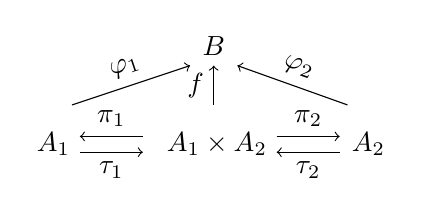
\begin{tikzpicture}
            \node [left] at (0,1) {$A_{1}$};
            \node [left] at (2.5,1) {$A_{1}\times A_{2}$};
            \node [left] at (4,1) {$A_{2}$};
            \draw [<-] (0,1.1)-- node [above, pos=0.5]{$\pi_{1}$} (0.8,1.1);
            \draw [->] (0,0.9)-- node [below, pos=0.5]{$\tau_{1}$} (0.8,0.9);
            \draw [->] (2.5,1.1)-- node [above, pos=0.5]{$\pi_{2}$} (3.3,1.1);
            \draw [<-] (2.5,0.9)-- node [below, pos=0.5]{$\tau_{2}$} (3.3,0.9);
            \node [above] at (1.7,2) {$B$};
            \draw [<-] (1.7,2)-- node [left, pos=0.5]{$f$} (1.7,1.5);
            \draw [<-] (1.4,2)-- node [above, pos=0.5, sloped]{$\varphi_{1}$} (-0.1,1.5);
            \draw [<-] (2,2)-- node [above, pos=0.5, sloped]{$\varphi_{2}$} (3.4,1.5);
        \end{tikzpicture}
    \end{figure}
    Next we verify the uniqueness. If there exist $f$ and $f'$ satisfies the condition, \[f(\tau_{1}(a_{1}))=f'(\tau_{1}(a_{1}))=f(a_{1},e)=f'(a_{1},e)\]\[f(\tau_{2}(a_{2}))=f'(\tau_{2}(a_{2}))=f(e,a_{2})=f'(e,a_{2})\]\[\begin{aligned}
        &f(\tau_{1}(a_{1}),\tau_{2}(a_{2}))=f(\tau_{1}(a_{1}))f(\tau_{2}(a_{2}))\\=&f'(\tau_{1}(a_{1}),\tau_{2}(a_{2}))=f'(\tau_{1}(a_{1}))f'(\tau_{2}(a_{2}))
    \end{aligned}\]
    so $f=f'$.
\end{answer}

$$ $$

\begin{ex}
    Every family $\{A_{i}|i\in I\}$ in the category of sets has a coproduct.
\end{ex}

\begin{answer}
    We examine $\bigcup\limits^{\cdot}A_{i}=\{(a,i)\in (\cup A_{i})\times I|a\in A_{i}\}$ which satisfies the condition. Define the morphism $\pi_{i}:A_{i}\to \bigcup\limits^{\cdot}A_{i}$ as $\pi_{i}(a)=(a,i)$. For any $B$ such that $\exists \varphi_{i}:A_{i}\to B$.
    
    \begin{figure}[H]\centering
        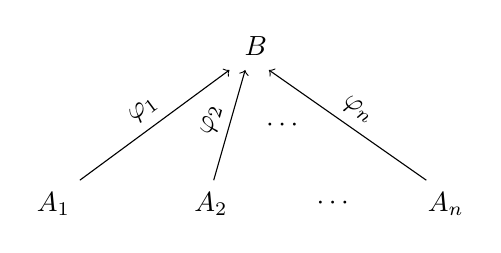
\begin{tikzpicture}
            \node [left] at (0,1) {$A_{1}$};
            \node [left] at (2,1) {$A_{2}$};
            \node [left] at (3.6,1) {$\cdots$};
            \node [left] at (5,1) {$A_{n}$};
            \node [left] at (2.5,3) {$B$};
            \draw [->] (0,1.3)-- node [above, pos=0.5, sloped]{$\varphi_{1}$} (1.9,2.7);
            \draw [->] (1.7,1.3)-- node [above, pos=0.5, sloped]{$\varphi_{2}$} (2.1,2.7);
            \draw [->] (4.4,1.3)-- node [above, pos=0.5, sloped]{$\varphi_{n}$} (2.4,2.7);
            \node [above] at (2.6,1.8) {$\cdots$};
        \end{tikzpicture}
    \end{figure}
    $\varphi(a)=x\in B$. Take $\varphi(a,i)=\varphi_{i}(a)$ defined on the subset of $\cup A_{i}\times I$, we can verify that the domain of $\varphi$ is $\bigcup\limits^{\cdot}A_{i}$. Then take $f=\varphi$, $f(\pi_{i}(a))=\varphi_{i}(a)$, $f\circ \pi_{i}=\varphi_{i}$.

    The uniqueness is obvious.
\end{answer}

$$ $$

\begin{ex}
    \begin{enumerate}[(a)]
        \item Show that in the category $\mathcal{S}_{*}$ of pointed sets product always exist; describe them.
        \item Show that in $\mathcal{S}_{*}$ every family of objects has a coproduct, describe the coproduct.
    \end{enumerate}
\end{ex}

\begin{answer}
    \begin{enumerate}[(a)]
        \item Define $\otimes$ as an operator between points and other elements in the pointed set. $\forall a\in A_{i}$, $a\otimes a_{i}=a_{1}\times a=a$. For a family of sets with their points $\{(A_{i},a_{i}|i\in I)\}$, consider $(A_{1}, A_{2}, \cdots, A_{n})=\{(a_{1}', a_{2}',\cdots, a_{n}')\}$. Define morphisms $\pi_{i}(a)=(a_{1}, a_{2},\cdots, a,\cdots, a_{n})$, $\pi_{i}:A_{i}\to (A_{1}, A_{2}, \cdots, A_{n})$.
        
        \begin{figure}[H]\centering
            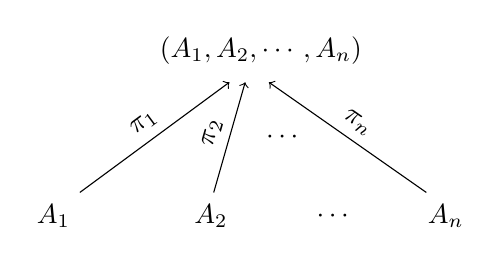
\begin{tikzpicture}
                \node [left] at (0,1) {$A_{1}$};
                \node [left] at (2,1) {$A_{2}$};
                \node [left] at (3.6,1) {$\cdots$};
                \node [left] at (5,1) {$A_{n}$};
                \node [above] at (2.3,2.8) {$(A_{1}, A_{2}, \cdots, A_{n})$};
                \draw [->] (0,1.3)-- node [above, pos=0.5, sloped]{$\pi_{1}$} (1.9,2.7);
                \draw [->] (1.7,1.3)-- node [above, pos=0.5, sloped]{$\pi_{2}$} (2.1,2.7);
                \draw [->] (4.4,1.3)-- node [above, pos=0.5, sloped]{$\pi_{n}$} (2.4,2.7);
                \node [above] at (2.6,1.8) {$\cdots$};
            \end{tikzpicture}
        \end{figure}
        For any $B$ such that $\exists \varphi_{i}:A_{i}\to B$.
    
        \begin{figure}[H]\centering
            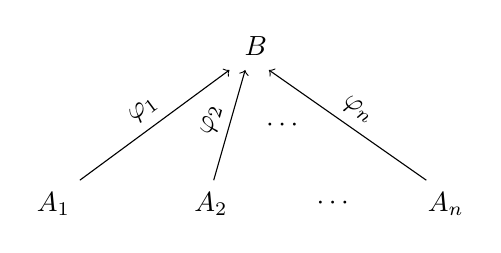
\begin{tikzpicture}
                \node [left] at (0,1) {$A_{1}$};
                \node [left] at (2,1) {$A_{2}$};
                \node [left] at (3.6,1) {$\cdots$};
                \node [left] at (5,1) {$A_{n}$};
                \node [left] at (2.5,3) {$B$};
                \draw [->] (0,1.3)-- node [above, pos=0.5, sloped]{$\varphi_{1}$} (1.9,2.7);
                \draw [->] (1.7,1.3)-- node [above, pos=0.5, sloped]{$\varphi_{2}$} (2.1,2.7);
                \draw [->] (4.4,1.3)-- node [above, pos=0.5, sloped]{$\varphi_{n}$} (2.4,2.7);
                \node [above] at (2.6,1.8) {$\cdots$};
            \end{tikzpicture}
        \end{figure}
        Take $f:(A_{1}, A_{2}, \cdots, A_{n})\to B$ as \[f(a_{1}',a_{2}',\cdots,a_{n}')=\varphi_{1}(a_{1}')\otimes\varphi_{2}(a_{2}')\otimes\cdots\otimes\varphi(a_{n}')\]Then $f\circ\pi_{i}(a)=f(a_{1},a_{2},\cdots,a,\cdots, a_{n})=\varphi_{1}(a_{1})\otimes\cdots\otimes\varphi_{i}(a)\otimes\cdots\otimes\varphi_{n}(a_{n})=\varphi_{i}(a)$. So $f\circ \pi_{i}=\varphi_{i}$.

        Next we verify the uniqueness. If there exist $f$ and $f'$ satisfies the condition. Then $\exists i\in I$ and $a\in A_{i}$ s.t. $f(a_{1},a_{2},\cdots,a,\cdots,a_{n})\neq f'(a_{1},a_{2},\cdots,a,\cdots,a_{n})$. But $f(\pi_{i}(a))=f'(\pi_{i}(a))$, so $f=f'$.
        \item The proof is similar to \textbf{Exercise 1.7.5}.
    \end{enumerate}
\end{answer}

$$ $$

\begin{ex}
    Let $F$ be a free object on a set $X(i:X\to F)$ in a concrete category $\mathcal{C}$. If $\mathcal{C}$ contains an object whose underlying set has at least two elements in it, then $i$ is an injective map of sets.
\end{ex}

\begin{answer}
    Assume $A\in\mathrm{obj}(\mathcal{C})$, $A$ has at least two elements and $X\xrightarrow{f} A$. $X\xrightarrow{i} F$ and $F$ is free on $X$, so there exists a morphism $\bar{f}$ s.t. $F\xrightarrow{\bar{f}}A$. If $\left| X \right|=1$, $i$ must be injective. For $\left| X \right| \geq 2$. Suppose $i$ is not injective. Take $x_{1}, x_{2}\in X$ and $i(x_{1})=i(x_{2})\in F$, $f(x_{1})=a_{1}$, $f(x_{2})=a_{2}$. $\bar{f}(i(x_{1}))=\bar{f}(i(x_{2}))=f(x_{1})=f(x_{2})=a_{1}=a_{2}$. That means all the elements in $A$ are identical. That's contradictory to the assumption.
\end{answer}

$$ $$

\begin{ex}
    Suppose $X$ is a set and $F$ is a free object on $X$ (with $i:X\to F$) in the category of groups. Prove that $i(X)$ is a set of generators for the group $F$.
\end{ex}

\begin{answer}
    Assume $G$ the subgroup of $F$ is the group generated by $i(X)$. Since $X\xrightarrow{i}G$ and $X\xrightarrow{i}F$, we can obtain unique morphism $\varphi$ such that $F\xrightarrow{\varphi}G$ and $\varphi \circ i=i$. 
    
    Consider morphism $1_{F}:F\to F$ which is the identical homomorphism. $F$ is free so $1_{F}$ is the unique homomorphism. Take $\subset:G\to F$ as a morphism defined as $\forall g\in G$, $\subset(g)=g$. Then
    
    \begin{figure}[H]\centering
        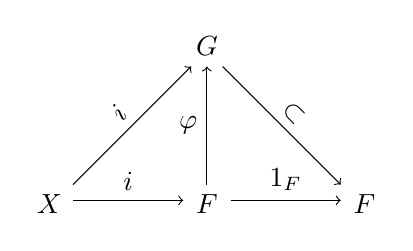
\begin{tikzpicture}
        \node [below] at (0,1) {$X$};
        \node [below] at (2,1) {$F$};
        \node [below] at (4,1) {$F$};
        \node [below] at (2,3) {$G$};
        \draw [->] (0.3,0.8)-- node [above, pos=0.5] {$i$} (1.7,0.8);
        \draw [->] (2.3,0.8)-- node [above, pos=0.5] {$1_{F}$} (3.7,0.8);
        \draw [->] (2,1)-- node [left, pos=0.5] {$\varphi$} (2,2.5);
        \draw [->] (0.3,1)-- node [above, pos=0.5, sloped] {$i$} (1.8,2.5);
        \draw [<-] (3.7,1)-- node [above, pos=0.5, sloped] {$\subset$} (2.2,2.5);
        \end{tikzpicture}
    \end{figure}
    $\subset\circ\varphi\circ i=1_{F}\circ i=i$ so $\subset\circ\varphi=1_{F}$. Thus $\subset$ is an epimorphism, $F\subset G$. So $F=G$ can be generated by $i(X)$.
\end{answer}
\section{Direct products and direct sums}
\begin{ex}
    $S_{3}$ is not the direct product of any family of its proper subgroups. The same is true of $Z_{p^{n}}$($p$ prime, $n\geq 1$) and $\mathbb{Z}$.
\end{ex}

$$ $$

\begin{ex}
    Give an example of groups $H_{i}$, $K_{i}$ such that $H_{1}\times H_{2}\cong K_{1}\times K_{2}$ and no $H_{i}$ is isomorphic to any $K_{j}$.
\end{ex}

$$ $$

\begin{ex}
    Let $G$ be and (additive) abelian group with subgroups $H$ and $K$. Show that $G\cong H\oplus K$ if and only if there are homomorphisms 
    
    \begin{figure}[H]\centering
        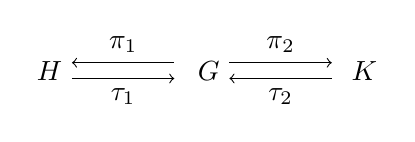
\begin{tikzpicture}
            \node [left] at (0,1) {$H$};
            \node [left] at (2,1) {$G$};
            \node [left] at (4,1) {$K$};
            \draw [<-] (0,1.1)-- node [above, pos=0.5]{$\pi_{1}$} (1.3,1.1);
            \draw [->] (0,0.9)-- node [below, pos=0.5]{$\tau_{1}$} (1.3,0.9);
            \draw [->] (2,1.1)-- node [above, pos=0.5]{$\pi_{2}$} (3.3,1.1);
            \draw [<-] (2,0.9)-- node [below, pos=0.5]{$\tau_{2}$} (3.3,0.9);
        \end{tikzpicture}
    \end{figure}
    such that $\pi_{1}\tau_{1}=1_{H}$, $\pi_{2}\tau_{2}=1_{K}$, $\pi_{1}\tau_{2}=0$ and $\pi_{2}\tau_{1}=0$, where 0 is the map sending every element onto the zero (identity) element, and $\tau_{1}\pi_{1}(x)+\tau_{2}\pi_{2}(x)=x$ for all $x\in G$.
\end{ex}

$$ $$

\begin{ex}
    Give an example to show that the weak direct product is not a coproduct in the category of all groups.
\end{ex}

$$ $$

\begin{ex}
    Let $G$, $H$ be finite cyclic groups. Then $G\times H$ is cyclic if and only if $(\left| G \right|, \left| H \right|  )=1$.
\end{ex}

$$ $$

\begin{ex}
    Every finitely generated abelian group $G\neq\left\langle e\right\rangle$ in which every element (except $e$) has order $p$ ($p$ prime) is isomorphic to $Z_{p}\oplus Z_{p}\oplus\cdots\oplus Z_{p}$($n$ summands) for some $n\geq 1$.
\end{ex}

$$ $$

\begin{ex}
    Let $H,K,N$ be nontrivial normal subgroups of a group $G$ and suppose $G=H\times K$. Prove that $N$ is in the center of $G$ or $N$ intersects one of $H,K$ nontrivially. Give examples to show that both possibilities can actually occur when $G$ is nonabelian.
\end{ex}

$$ $$

\begin{ex}
    Corollary 8.7 is false if one of the $N_{i}$ is not normal.
\end{ex}

$$ $$

\begin{ex}
    If a group $G$ is the (internal) direct product of its subgroups $H$, $K$, then $H\cong G / K$ and $G /H \cong K$.
\end{ex}

$$ $$

\begin{ex}
    If $\{G_{i}|i\in I\}$ is a family of groups, then $\prod^{w}G_{i}$ is the internal weak product its subgroups $\{\tau_{i}(G_{i})|i\in I\}$.
\end{ex}

$$ $$

\begin{ex}
    Let $\{N_{i}|i\in I\}$ be a family of subgroups of a group $G$. Then $G$ is the internal weak product of $\{N_{i}|i\in I\}$if and only if:
    \begin{enumerate}[(i)]
        \item $a_{i}a_{j}=a_{j}a_{i}$ for all $i\neq j$ and $a_{i}\in N_{i}$, $a_{j}\in N_{j}$;
        \item every nonidentity element of $G$ is uniquely a product $a_{i_{1}}\cdots a_{i_{n}}$, where $i_{i},\dots,i_{n}$ are distinct elements of $I$ and $e\neq a_{i_{k}}\in N_{i_{k}}$ for each $k$.
    \end{enumerate}
\end{ex}

$$ $$

\begin{ex}
    A normal subgroup $H$ of a group $G$ is said to be a \textbf{direct factor} (\textbf{direct summand} if $G$ is additive abelian) if there exists a (normal) subgroup $K$ of $G$ such that $G=H\times K$.
    \begin{enumerate}[(a)]
        \item If $H$ is a direct factor of $K$ and $K$ is a direct factor of $G$, then $H$ is normal in $G$.
        \item If $H$ is a direct factor of $G$, then every homomorphism $H\to G$ may be extended to an endomorphism $G\to G$. However, a monomorphism $H\to G$ need not be extendible to and automorphism $G\to G$.
    \end{enumerate}
\end{ex}

$$ $$

\begin{ex}
    Let $\{G_{i}|i\in I\}$ be a family of groups and $J\subset I$. The map $\alpha: \prod\limits_{j\in J}G_{j}\to \prod\limits_{i\in I}G_{i}$ given by $\{a_{j}\}\mapsto \{b_{i}\}$, where $b_{j}=a_{j}$ for $j\in J$ and $b_{i}=e_{i}$(identity in $G_{i}$) for $i\notin J$, is a monomorphism of groups and $\prod\limits_{i\in I}G_{i} /\alpha(\prod\limits_{j\in J}G_{j})\cong \prod\limits_{i\in I-J}G_{i}$.
\end{ex}

$$ $$

\begin{ex}
    For $i=1,2$ let $H_{i}\lhd G_{i}$ and give examples to show that each of the following statements may be false:
    \begin{enumerate}[(a)]
        \item $G_{1}\cong G_{2}$ and $H_{1}\cong H_{2}\Rightarrow G_{1} /H_{1}\cong G_{2} /H_{2}$.
        \item $G_{1}\cong G_{2}$ and $G_{1}/ H_{1}\cong G_{2} / H_{2}\Rightarrow H_{1}\cong H_{2}$.
        \item $H_{1}\cong H_{2}$ and $G_{1}/ H_{1}\cong G_{2} / H_{2}\Rightarrow G_{1}\cong G_{2}$.
    \end{enumerate}
\end{ex}
\section{Free groups, free products, generators and relations}
\begin{ex}
    Every nonidentity elements in a free group $F$ has a infinite order.
\end{ex}

\begin{answer}
    Define the length of a word $x=a_{1}^{\lambda_{1}}a_{2}^{\lambda_{2}}\cdots a_{n}^{\lambda_{n}}$ is $n$ and denote it as $len(x)$. Assume $len(x)=n$ for some $n\in F$ and $len(1)=0$, we prove that $len(x^{m})\geq n\forall m\geq 1$.

    Let $k$ be the largest integer such that  $a_{n-j}^{\lambda_{n-j}}=a_{n}^{-\lambda_{j}}$ for $j=0, 1, \dots, k-1$. If $k>\left[\frac{n}{2}\right]$. For even $k$, $a_{\frac{n}{2}}^{\lambda_{\frac{n}{2}}}=a_{\frac{n}{2}+1}^{-(\lambda_{\frac{n}{2}+1})}$, $a_{\frac{n}{2}-1}^{\lambda_{\frac{n}{2}-1}}=a_{\frac{n}{2}+2}^{-(\lambda_{\frac{n}{2}+2})}$, $\cdots$ which means $x=a_{1}^{\lambda_{1}}a_{2}^{\lambda_{2}}\cdots a_{n}^{\lambda_{n}}=1$. For odd $k$, $a_{\left[\frac{n}{2}\right]+1}^{\lambda_{\left[\frac{n}{2}\right]+1}}=a_{\left[\frac{n}{2}\right]+1}^{-(\lambda_{\left[\frac{n}{2}\right]+1})}$, which is contradictory to $x$ is reduced. So $k\leq \left[\frac{n}{2}\right]$.

    Divide $x=x_{1}x_{2}x_{3}$ where $x_{1}=a_{1}^{\lambda_{1}}\cdots a_{k}^{\lambda_{k}}$, $x_{2}=a_{k+1}^{\lambda_{k+1}}\cdots a_{n-k}^{\lambda_{n-k}}$, $x_{3}=a_{n-k+1}^{\lambda_{n-k+1}}\cdots a_{n}^{\lambda_{n}}$. $x_{3}x_{1}=1$. So $len(x)=len(x_{1})+len(x_{2})+len(x_{3})=n$. $x^{m}=x_{1}x_{2}x_{3}x_{1}x_{2}x_{3}\cdots x_{1}x_{2}x_{3}=x_{1}x_{2}^{m}x_{3}$. $len(x^{m})=len(x_{1})+m\cdot len(x_{2})+len(x_{3})\geq n$. So $\forall m\geq 1$, $x^{m}\neq 1$, $\left| x \right| $ is infinite.
\end{answer}

$$ $$

\begin{ex}
    Show that the free group on the set $\{a\}$ is an infinite cyclic group, and hence isomorphic to $\mathbf{Z}$.
\end{ex}

\begin{answer}
    $F(\{a\})=\left\langle a\right\rangle$ and thus it's a infinite cyclic group. $F(\{a\})\cong \mathbf{Z}$.
\end{answer}

$$ $$

\begin{ex}
    Let $F$ be a free group and let $N$ be the subgroup generated by the set $\{x^{n}|x\in F, n\text{ a fixed integer}\}$. Show that $N\lhd F$.
\end{ex}

$$ $$

\begin{ex}
    Let $F$ be the free group on the set $X$, and let $Y\subset H$. If $H$ is the smallest normal subgroup of $F$ containin $Y$, then $F /H$ is a free group.
\end{ex}

$$ $$

\begin{ex}
    The group defined by generators $a,b$ and relations $a^{8}=b^{2}a^{4}=ab^{-1}ab=e$ has order at most 16.
\end{ex}

$$ $$

\begin{ex}
    The cyclic group of order 6 is the group defined by generators $a, b$ and relations $a^{2}=b^{3}=a^{-1}b^{-1}ab=e$.
\end{ex}

$$ $$

\begin{ex}
    Show that the group defined by generators $a, b$ and relations $a^{2}=e$, $b^{3}=e$ is infinite and nonabelian.
\end{ex}

$$ $$

\begin{ex}
    The group defined by generators $a, b$ and relations $a^{n}=e (3\leq n\in \mathbf{N}^{*})$, $b^{2}=e$ and $abab=e$ is the dihedral group $D_{n}$.
\end{ex}

$$ $$

\begin{ex}
    The group defined by the generator $b$ and $b^{m}=e(m\in \mathbf{N}^{*})$ is the cyclic group $Z_{m}$.
\end{ex}

$$ $$

\begin{ex}
    The operation of free product is commutative and associative: for any groups $A$, $B$, $C$, $A*B\cong B*A$ and $A*(B*C)\cong (A*B)*C$.
\end{ex}

$$ $$

\begin{ex}
    If $N$ is normal subgroup of $A*B$ generated by $A$, then $(A*B) /N\cong B$.
\end{ex}

$$ $$

\begin{ex}
    If $G$ and $H$ each have more than one element, then $G*H$ is an infinite group with center $\left\langle e\right\rangle$.
\end{ex}

$$ $$

\begin{ex}
    A free group is a free product of infinite cyclic groups.
\end{ex}

$$ $$

\begin{ex}
    If $G$ is the group defined by generators $a, b$ and relations $a^{2}=e$, $b^{3}=e$, then $G\cong Z_{2}*Z_{3}$.
\end{ex}

$$ $$

\begin{ex}
    If $f:G_{1}\to G_{2}$ and $g:H_{1}\to H_{2}$ are homomorphisms of groups, then there is a unique homomorphism $h:G_{1}*H_{1}\to G_{2}H_{2}$ such that $h|G_{1}=f$ and $h|H_{1}=g$.
\end{ex}

\chapter{The structure of groups}

\chapter{Rings}
\section{Sequence and their Limits}
\begin{definition}
    We call $A$ is the \textbf{limit} of a sequence, if for any neighborhood $V(A)$ around $A$, there exists a serial number $N$ (related to $V(A)$), any item has serial number larger than which will be contained in $V(A)$.
\end{definition}
Now we give the rigorous definition of limit of a sequence:\

\begin{definition}
    $A\in R$ is a limit of a sequence, if for any $\varepsilon >0$, there exists a number $N$, for all $n>N$, $\left\lvert x_{n}-A\right\lvert<\varepsilon$.    
\end{definition}

Denotion $\lim\limits_{n \to \infty}x_{n}\to A$ are used to indicate the limit of $\{x_{n}\}$.
\[\left(\lim\limits_{n \to \infty}x_{n}=A\right):=\forall V(A)\ \exists N\in \mathbb{N}\ \forall n>N\ (x_{n}\in V(A)) \]
or
\[\left(\lim\limits_{n \to \infty}x_{n}=A\right):=\forall \varepsilon>0\ \exists N\in \mathbb{N}\ \forall n>\mathbb{N}\ (\left| x_{n}-A \right|<\varepsilon )\]

\begin{definition}
    If $\lim\limits_{n \to \infty}x_{n}=A$, we say that $\{x_{n}\}$ converges to or tend to $A$. We call it the convergent sequences. The sequences doesn't have a limit is named divergent sequence.
\end{definition}
\section{Ideals}
\begin{ex}
    The set of all nilpotent elements in a commutative ring forms an ideal.
\end{ex}

\begin{answer}
    Assume the set is $I$, then $\forall a,b\in I$, $a^{m}=b^{n}=0$, $(a+b)^{m+n}=0$ and $(ab)^{mn}=0$ so $a+b\in I$, $ab\in I$. $I$ is a subring. $\forall x\in R$, $(xa)^{m}=x^{m}a^{m}=0$, $(ax)^{m}=a^{m}x^{m}=0$, so $xa\in I$ and $ax\in I$, $I$ is an ideal.
\end{answer}

$$ $$

\begin{ex}
    Let $I$ be an ideal in a commutative ring $R$ and let $\mathrm{Rad} I=\{r\in R| r^{n}\in I \text{ for some } n\}$. Show that $\mathrm{Rad}I$ is an ideal.
\end{ex}

\begin{answer}
    $\mathrm{Rad} I$ is a ring since $R$ is a commutative ring. For $r\in \mathrm{Rad} I$ and $\forall x\in R$, $(xr)^{n}=x^{n}r^{n}\in I$ so $xr\in \mathrm{Rad} I$, $(rx)^{n}=r^{n}x^{n}\in I$ so $rx\in \mathrm{Rad} I$. Thus $\mathrm{Rad} I$ is an ideal.
\end{answer}

$$ $$

\begin{ex}
    If $R$ is a ring and $a\in R$, then $J=\{r\in R|ra=0\}$ is a left ideal and $K=\{r\in R|ar=0\}$ is a right ideal in $R$.
\end{ex}

\begin{answer}
    $J$ is a subring of $R$. For $r\in J$ and $\forall x\in R$, $(xr)a=x(ra)=0$ so $xr\in J$, $J$ is a left ideal. Similarly, $I$ is a right ideal.
\end{answer}

$$ $$

\begin{ex}
    If $I$ is a left ideal of $R$, then $A(I)=\{r\in R|rx=0 \text{ for every }x\in I\}$ is an ideal in $R$.
\end{ex}

\begin{answer}
    For any $a,b\in A(I)$, we have $ab\in A(I)$ and $a+b\in A(I)$. For $r\in A(I)$ and $\forall x\in R$, $(xr)x'=x(rx')=0$ for every $x'\in I$, so $xr\in A(I)$. $(rx)x'=r(xx')$, $x x'\in I$ so $rx x'=0$, $rx\in A(I)$. Thus $A(I)$ is an ideal of $R$.
\end{answer}

$$ $$

\begin{ex}
    If $I$ is an ideal in a ring $R$, let $\left[R:I\right]=\{r\in R|xr\in I \text{ for every }x\in R\}$. Prove that $\left[ R:I\right]$ is an ideal of $R$ which contains $I$.
\end{ex}

\begin{answer}
    $I$ is a subring of $R$ so $\left[R:I\right]$ is also a subring of $R$. For $r\in\left[R:I\right]$ and $x, x'\in R$, $x'xr=(x'x)r\in I$ so $xr\in \left[R:I\right]$, $x'rx=(x'r)x\in I$ so $rx\in \left[R:I\right]$. $\left[R:I\right]$ is an ideal of $R$. Since $\forall r\in I$, $xr\in I$ and $rx\in I$, $I\subset \left[R:I\right]$.
\end{answer}

$$ $$

\begin{ex}
    \begin{enumerate}[(a)]
        \item The center of the ring $S$ of all $2\times 2$ matrices over a field $F$ consists of all matrices of the form $\begin{pmatrix}
            a&0\\0&a
        \end{pmatrix}$.
        \item Then center of $S$ is not an ideal in $S$.
        \item What is the center of the ring of all $n\times n$ matrices over a division ring?
    \end{enumerate}
\end{ex}

\begin{answer}
    \begin{enumerate}[(a)]
        \item $\forall x\in M_{F}(2,2)$, $x=\begin{pmatrix}
            x_{1}&x_{2}\\x_{3}&x_{4}
        \end{pmatrix}$\[x\begin{pmatrix}
            a&0\\0&a
        \end{pmatrix}=\begin{pmatrix}
            a&0\\0&a
        \end{pmatrix}x=\begin{pmatrix}
            ax_{1}&ax_{2}\\ax_{3}&ax_{4}
        \end{pmatrix}\] so $\begin{pmatrix}
            a&0\\0&a
        \end{pmatrix}\in C(M_{F}(2,2))$.

        $\forall \begin{pmatrix}
            a_{1}&a_{2}\\a_{3}&a_{4}
        \end{pmatrix}\in C(M_{F}(2,2))$, take $\begin{pmatrix}
            0&1_{F}\\0&0
        \end{pmatrix}\in M_{F}(2,2)$\[\begin{pmatrix}
            a_{1}&a_{2}\\a_{3}&a_{4}
        \end{pmatrix}\begin{pmatrix}
            1_{F}&0\\0&0
        \end{pmatrix}=\begin{pmatrix}
            a_{1}&0\\a_{3}&0
        \end{pmatrix}\]\[\begin{pmatrix}
            1_{F}&0\\0&0
        \end{pmatrix}\begin{pmatrix}
            a_{1}&a_{2}\\a_{3}&a_{4}
        \end{pmatrix}=\begin{pmatrix}
            a_{1}&a_{2}\\0&0
        \end{pmatrix}\] so $a_{2}=a_{3}=0$.
        \[\begin{pmatrix}
            a_{1}&a_{2}\\a_{3}&a_{4}
        \end{pmatrix}\begin{pmatrix}
            0&1_{F}\\0&0
        \end{pmatrix}=\begin{pmatrix}
            0&a_{1}\\0&a_{3}
        \end{pmatrix}\]\[\begin{pmatrix}
            0&1_{F}\\0&0
        \end{pmatrix}\begin{pmatrix}
            a_{1}&a_{2}\\a_{3}&a_{4}
        \end{pmatrix}\begin{pmatrix}
            a_{3}&a_{4}\\0&0
        \end{pmatrix}\] so $a_{1}=a_{4}$. All the elements of $C(M_{F}(2,2))$ has the form $\begin{pmatrix}
            a&0\\0&a
        \end{pmatrix}$.
        \item For $c\in C(S)$. If $S$ is not commutative, $\forall x,x'\in R$, we need $xc\in C(S)\Rightarrow x'xc=xcx'=xx'c$, however, this may not always true.
        \item By multiplying $\begin{pmatrix}
            1_{F}& &\\ &\ddots & \\ & &0
        \end{pmatrix}$, $\begin{pmatrix}
            0& & &\\ &1_{F}& &\\ & &\ddots&\\ & & &0
        \end{pmatrix}$, $\dots$, $\begin{pmatrix}
            0& &\\ &\ddots & \\ & &1_{F}
        \end{pmatrix}$, we can have $C(M_{F}(2,2))$ consist of all the elements in the form of $a\begin{pmatrix}
            1_{F}& & &\\ &1_{F}& &\\ & &\ddots&\\ & & &1_{F}
        \end{pmatrix}$.
    \end{enumerate}
\end{answer}
$$ $$

\begin{ex}
    \begin{enumerate}[(a)]
        \item A ring $R$ with identity is a division ring if and only if $R$ has no proper left ideals.
        \item If $S$ is a ring (possibly without identity) with no proper left ideals, then either $S^{2}=0$ or $S$ is a division ring.
    \end{enumerate}
\end{ex}

\begin{answer}
    \begin{enumerate}[(a)]
        \item Suppose not. $I$ is an ideal in $R$. $\forall r\in I$, take $r^{-1}\in R$, then $1_{R}\in I$ so $I=R$ is not a  proper ideal.
        \item $I=\{a\in S|Sa=0\}$ is a left ideal since $\forall x,x'\in S$, $x'(xs)=(x'x)s=0$, $xs\in I$. Thus $I=0$ or $I=S$. If $I=S$, then $S^{2}=0$. If $I=0$, we prove $S$ has no zero divisor.
        
        For the set $I'=\{r\in S|rb=0\}$, $I'\subset I$. $I'$ is a subring of $S$, and $I'$ is also a left ideal of $S$. So $I'=0$, $b$ has no left zero divisors. $\forall a\in S$, $Sa$ is a left ideal of $S$. $Sa\neq 0$ so $Sa=S$. Thus, $\exists 1_{S}\in S$, such that $1_{S}a=a$. Since $s_{1}-s_{2}$ has no left zero divisor, $as_{1}=as_{2}\Rightarrow s_{1}=s_{2}$. So $aS=S$. For all $s\in S$, $\exists s'$ s.t. $s=as'$ so $\forall s\in S$, $1_{S}\cdot s=1_{S}as'=as'=s$. $aS=S$ so $\exists 1_{S}'\in S$, $a1_{S}'=a$. Similarly, $\forall s\in S$, $s1_{S}=s$. Then $1_{S}1_{S}'=1_{S}=1_{S}'$ so $S$ has identity. Since $Sa=aS=S$, we can have $S$ is a division ring.
    \end{enumerate}
\end{answer}

$$ $$

\begin{ex}
    Let $R$ be a ring with identity and $S$ the ring of all $n\times n$ matrices over $R$. $J$ is an ideals of $S$ if and only if $J$ is the ring of all $n\times n$ matrices over $I$ for some ideal $I$ in $R$.
\end{ex}

\begin{answer}
    If $J$ is an ideal. Denote $E_{r,s}$ as the matrix which has $1_{R}$ as the $r$ column and $s$ row. Then $\forall A=(a_{ij})$, $E_{p,r}AE_{s,q}$ is a matrix with $a_{rs}$ in the $p$ column and  $q$ row. So for $A\in J$ $(aE_{p,r})A(bE_{s,q})$ is the matrix with $aa_{rs}b$ in the $p$ column and  $q$ row. $aa_{rs}b\in I$. Then because of closure we know $J$ contains all $n\times n$ matrices over $I$. 

    If $J$ consists of all $n\times n$ matrices over $I$, the proof is trivial.
\end{answer}

$$ $$

\begin{ex}
    Let $S$ be the ring of all $n\times n$ matrices over a division ring $D$.
    \begin{enumerate}[(a)]
        \item $S$ has no proper ideals (that is, 0 is the maximal ideal).
        \item $S$ has zero divisors. Consequently, (i) $S\cong S /0$ is not a division ring and (ii) 0 is a prime ideal which does not satisfy condition (1) of Theorem 2.15.
    \end{enumerate}
\end{ex}

\begin{answer}
    \begin{enumerate}[(a)]
        \item $J$ is an ideal of $S$ so $J$ consists of all $n\times n$ matrices over $I$ where $I$ is an ideal of $D$. From \textbf{Exercise 3.2.7}, $D$ has no proper ideal so $I=0\Rightarrow J=0$.
        \item For $A=(a_{ij})$ with $a_{ri}=0$ for $i=1,2\cdots$ and other entries doesn't equals to zero, we have $E_{1r}A=0$. $S$ has no zero divisors.
    \end{enumerate}
\end{answer}

$$ $$

\begin{ex}
    \begin{enumerate}[(a)]
        \item Show that $\mathbf{Z}$ is a principle ideal ring.
        \item Every homomorphic image of a principle ideal ring is also a principle ideal ring.
        \item $Z_{m}$ is a principle ideal ring for every $m>0$.
    \end{enumerate}
\end{ex}

\begin{answer}
    \begin{enumerate}[(a)]
        \item For any ideal $I$ in $\mathbf{Z}$, $I$ is a subring so $I=m\mathbf{Z}$ where $m\in \mathbf{Z}$. $m\mathbf{Z}=(m)$ is a principle ideal so $\mathbf{Z}$ is a PID.
        \item For $f:R\to S$ with $f(r)=s$ and $R$ is a principle ideal ring. Consider $f:R\to \mathrm{Im}f\subset S$. For any ideal $J\subset \mathrm{Im}f$, $f^{-1}(J)$ is an ideal since $\forall a\in f^{-1}(J)$ and $r\in R$, $f(ar)=f(a)f(r)\in J\Rightarrow ar\in f^{-1}(J)$. $f^{-1}(J)$ is a principle ideal, assume $f^{-1}(J)=(a)$. Then $\forall r\in R$, $ar\in (a)$, $ra\in (a)$. $f(ar)=f(a)f(r)\in J$ and $f(ra)=f(r)f(a)\in J$ since $f(a)\in J$ and $f(r)\in S$. So $(f(a))\subset J$. $J=f((a))=\{f(ra+as+na+\sum\limits_{i=1}^{m}r_{i}as_{i})| r, s, r_{i}, s_{i}\in R, n\in \mathbf{Z}\}=\{f(r)f(a)+f(a)f(s)+nf(a)+\sum\limits_{i=1}^{m}f(r_{i})f(a_{i})f(s_{i})| r, s, r_{i}, s_{i}\in R, n\in \mathbf{Z}\}\subset (f(a))$. So $J=(f(a))$ is a principle ideal. The image of a principle ideal ring is also a principle ideal ring.
    \end{enumerate}
\end{answer}

$$ $$

\begin{ex}
    If $N$ is the ideal of all nilpotent elements in a commutative ring $R$, then $R /N$ is a ring with no nonzero nilpotent elements.
\end{ex}

\begin{answer}
    Suppose not. $\exists r\in R$, $r\notin N$, $(r+N)^{n}=0$ for some $n\in\mathbf{N}$. \[(r+N)^{n}=r^{n}+N=N\Rightarrow r^{n}\in N\]so for some $m\in \mathbf{N}$, $r^{nm}=0\Rightarrow r\in N$. That's contradictory!
\end{answer}

$$ $$

\begin{ex}
    Let $R$ be a ring without identity and with no zero divisors. Let $S$ be the ring whose additive group is $R\times \mathbf{Z}$ as in the proof of Theorem 1.10. Let $A=\{(r,n)\in S|rx+nx=0 \text{ for every }x\in R\}$.
    \begin{enumerate}[(a)]
        \item $A$ is an ideal in $S$.
        \item $S /A$ has an identity and contains a subring isomorphic to $R$.
        \item $S /A$ has no zero divisors.
    \end{enumerate}
\end{ex}

\begin{answer}
    \begin{enumerate}[(a)]
        \item For $(r,n), (r',n')\in S$, $(r'+r)x+(n'+j)x=rx+nx+r'x+n'x=0$, so $(r+r',n+n')\in A$. $(r,n)(r'n')=(rr'+nr'+n'r,nn')$, $rr'x+n'rx+nr'x+nn'x=r(r'x+n'x)+n(r'x+n'x)=0$, so $(r,n)(r',n')\in A$. $A$ is a subring of $R\times \mathbf{Z}$. $\forall (r_{1},n_{1})\in R\times \mathbf{Z}$, $(r_{1},n_{1})(r,n)=(r_{1}r+nr_{1}+n_{1}r,nn_{1})\Rightarrow r_{1}rx+nr_{1}x+n_{1}rx+nn_{1}x=r_{1}(rx+nx)+n_{1}(rx+nx)=0\Rightarrow (r_{1},n_{1})(r,n)\in A$. $A$ is an ideal of $R\times \mathbf{Z}$.
        \item Take $0_{R}\in R$ and $(0_{R},1)\in S$. Then $(0_{R},1)+A$ is an identity of $S /A$. \[\forall (r,n)\in S, \quad (r,n)(0_{R},1)=(0_{R},1)(r,n)=(r,n)\]
        \item For any $(r,n), (s,m)$ satisfy that $(r,n)(s,m)\in A$, we prove that $(r,n)\in A$ or $(s,m)\in A$. Suppose $sx+mx\neq 0$, $r(sx+mx)+n(sx+mx)=0\Rightarrow (sx+mx)r(sx+mx)+n(sx+mx)^{2}=0\Rightarrow ((sx+mx)r+n(sx+mx))(sx+mx)=0\Rightarrow (sx+mx)r+n(sx+mx)=0$. For any $x\in R$, $(sx+mx)rx+n(sx+mx)x=0\Rightarrow(sx+mx)(rx+nx)=0\Rightarrow rx+nx=0$, so $(r,n)\in A$. $S /A$ has no divisor.
    \end{enumerate}
\end{answer}

$$ $$

\begin{ex}
    Let $f:R\to S$ be a homomorphism of rings, $I$ and ideal in $R$, and $J$ an ideal in $S$.
    \begin{enumerate}[(a)]
        \item $f^{-1}(J)$ is and ideal in $R$ that contains $\mathrm{Ker}f$.
        \item If $f$ is an epimorphism, then $f(I)$ is an ideal in $S$. If $f$ is not surjective, $f(I)$ need not be an ideal.
    \end{enumerate}
\end{ex}

\begin{answer}
    \begin{enumerate}[(a)]
        \item $\forall a\in f^{-1}(J)$ and $r\in R$, $f(ar)=f(a)f(r)\in J\Rightarrow ar\in J$. Similarly, $ra\in J$, $f^{-1}(J)$ is an ideal. $\mathrm{Ker}f\subset f^{-1}(J)$ since $0_{S}\in J$.
        \item $\forall b\in f(I)$ and $s\in S$, $f$ is a epimorphism so $s=f(r)$, $b=f(a)$ for some $r, a\in R$. $sb=f(r)f(a)=f(ar)$, $ar\in I\Rightarrow sb\in f(I)$, similarly $bs\in f(I)$. $f(I)$ is an ideal.
        
        If $f$ is not surjective. Take $Z\left[x\right]$ and $\mathbf{Z}$ which is a subring but not an ideal in $Z\left[x\right]$. $\mathbf{Z}$ is an ideal of itself, $f=1_{\mathbf{Z}}$ satisfies the condition.
    \end{enumerate}
\end{answer}

$$ $$

\begin{ex}
    If $P$ is an ideal in a not necessarily commutative ring $R$, then the following conditions are equivalent.
    \begin{enumerate}[(a)]
        \item $P$ is a prime ideal.
        \item If $r,s\in R$ are such that $rRs\subset R$, then $r\in P$ or $s\in P$.
        \item If $(r)$ and $(s)$ are principle ideals of $R$ such that $(r)(s)\subset P$, then $r\in P$ or $s\in P$.
        \item If $U$ and $V$ are right ideals in $R$ such that $UV\subset R$, then $U\subset R$ or $V\subset R$.
        \item If $U$ and $V$ are left ideals in $R$ such that $UV\subset R$, then $U\subset R$ or $V\subset R$.
    \end{enumerate}
\end{ex}

$$ $$

\begin{ex}
    The set consisting of zero and all zero divisors in a commutative ring with identity contains at least one prime ideal.
\end{ex}

\begin{answer}
    Denote $S=R-Z$. $\forall a,b\in S$, we prove that $ab\in S$. Suppose $\exists (ab)c=0$ for some $c\in R$, $a$, $b$ are not zero divisors so $abc=b(ac)=a(bc)=0$, so $ac=0$, $bc=0\Rightarrow c=0$, so $ab$ is not a zero divisor. Thus $Z=R-S$ contains an prime ideal.
\end{answer}

$$ $$

\begin{ex}
    Let $R$ be a commutative ring with identity and suppose that the ideal $A$ of $R$ is contained in a finite union of prime ideals $P_{1}\cup\cdots\cup P_{n}$. Show that $A\subset P_{i}$ for some $i$.
\end{ex}

\begin{answer}
    Suppose not. We choose the smallest $I$ such that for all $i\in I$, $P_{i}\cap A\neq \varnothing$ and $A\cap P_{i}\not\subset\bigcup\limits_{j\neq i}P_{j}$ for any $i\in I$. So $\exists a_{i}\in (A\cap P_{i})-(\bigcup\limits_{j\neq i}P_{j})$, $\forall i\in I$. Take $x=a_{1}+a_{2}a_{3}\cdots a_{n}$, $x\in A$ since $a_{i}\in A$ for all $i\in I$. And $x\notin P_{i}$ for $i=2,3,\dots, n$ since $a_{1}\notin P_{i}$, $i=2,3,\dots, n$. $x\notin P_{1}$ since $P_{1}$ is prime and $a_{2}, \dots, a_{n}\notin P_{1}$. So $x\notin \bigcup\limits_{j\neq i}P_{j}$, which is contradictory!
\end{answer}

$$ $$

\begin{ex}
    Let $f:R\to S$ be an epimorphism of rings with kernel $K$.
    \begin{enumerate}[(a)]
        \item If $P$ is a prime ideal in $R$ that contains $K$, then $f(P)$ is a prime ideal in $S$.
        \item If $Q$ is a prime ideal in $S$, then $f^{-1}(Q)$ is a prime ideal in $R$ that contains $K$.
        \item There is a one-to-one correspondence between the set of all prime ideals in $R$ that contain $K$ and the set of all prime ideals in $S$, given by $P\mapsto f(P)$.
        \item If $I$ is an ideal in a ring $R$, then every prime ideal in $R /I$ is of the form $P /I$, where $P$ is a prime ideal in $R$ that contains $I$.
    \end{enumerate}
\end{ex}

\begin{answer}
    \begin{enumerate}[(a)]
        \item From \textbf{Exercise 3.2.13} we know $f(P)$ is an ideal. $\forall x,y\in f(P)$, $\exists a.b\in R$, $x=f(a)$, $y=f(b)$ and $a,b\notin P$. Assume $\exists p\in P$ such that $f(ab)=f(p)$, then $f(ab-p)=0$, $ab-p\in\mathrm{Ker}f\subset P\Rightarrow ab\in P$. That's contradictory to $a,b\notin P$ so $xy\notin f(P)$. $f(P)$ is prime.
        \item From \textbf{Exercise 3.2.13}, $f^{-1}(Q)$ is an ideal. Take $g:S\to S /Q$ and $gf:R\to S /Q$. By the Theorem of homomorphism, $R /f^{-1}(Q) \cong S /Q$ is a ring without divisor, so $f^{-1}(Q)$ is prime.
        \item From (a), (b), $f$ is a one-to-one map between prime ideals given by $P\mapsto f(P)$.
        \item Consider the homomorphism $f:R\to R /I$. For any prime ideal $P\subset R$ and $f(P)$ is an prime ideal in $R$, $\mathrm{Ker}f=I$ so for prime ideals $I\subset P\subset R$. $P$ can have one to one correspondence with $f(P)=P /I\subset R/I$. So all the prime ideals has the form $P /I$.
    \end{enumerate}
\end{answer}

$$ $$

\begin{ex}
    An ideal $M\neq R$ in a commutative ring $R$ with identity is maximal if and only if for every $r\in R-M$, there exists $x\in R$ such that $1_{R}-rx\in M$.
\end{ex}

\begin{answer}
    If $M$ is maximal, then $M$ is prime. So $rR+M=R$, $r(R-M)+M=R$ and $r(R-M)\cap M=\varnothing$. Take $1_{R}\in R$ we have $x\in R-M$, $1_{R}-xr\in M$. If $\forall r\in R-M$, $\exists x\in R$ such that $1_{R}-rx\in M$. Suppose $M\subset I\subset R$ where $I$ is an ideal, $I\neq R$ so $1_{R}\notin R$. Take $r\in I-M\subset R-M$, then $\forall x\in R$, $rx\in I$, so $1_{R}-rx\notin I$ thus $1_{R}-rx\notin M$. That's contradictory!
\end{answer}

$$ $$

\begin{ex}
    The ring $E$ of even integers contains a maximal ideal $M$ such that $E /M$ is not a field.
\end{ex}

\begin{answer}
    $E=2\mathbf{Z}$ and $M$ is a maximal ideal in $E$ and for any subring of $E$ has the form $wn\mathbf{Z}$ where $n\in \mathbf{Z}$. $2n\mathbf{Z}$ is an ideal in $2\mathbf{Z}$. Take $n=15$, $(2,15)=1$ so $2\mathbf{Z} /30\mathbf{Z}\cong \mathbf{Z} /15\mathbf{Z}$ which is not a field since $3\cdot 5=0$ is a zero divisor.
\end{answer}

$$ $$

\begin{ex}
    In the ring $\mathbf{Z}$ the following conditions on a nonzero ideal $I$ are equivalent: (i) $I$ is prime; (ii) $I$ is maximal; (iii) $I=(p)$ with $p$ prime.    
\end{ex}

\begin{answer}
    $\mathbf{Z}$ is an integer domain so (ii)$\Rightarrow$(i).

    (i)$\Rightarrow$(iii): Trivial.

    (iii)$\Rightarrow$(ii): For any $n\notin (p)$, we have $p\nmid n$ thus $\exists x,y\in \mathbf{Z}$ such that $px+my=1$. Consider an ideal $I$ and $(p)\subset I$, $n\in I$, then $1\in I$ so $I=\mathbf{Z}$ which means $(p)$ is maximal.
\end{answer}

$$ $$

\begin{ex}
    Determine all prime and maximal ideals in the ring $Z_{m}$.
\end{ex}

\begin{answer}
    $Z_{m}^{2}=Z_{m}$ so every maximal ideal is prime in $Z_{m}$. $Z_{m}\cong \mathbf{Z} /m\mathbf{Z}$ via $\varphi:\bar{x}\mapsto mz+x$. From \textbf{Exercise 3.2.17}, all the prime ideals in $\mathbf{Z}/m\mathbf{Z}$ are $P /m\mathbf{Z}$, where $P$ is a prime ideal contains $m\mathbf{Z}=(m)$.

    If $m$ is prime, $(m)$ is prime, too. So no such ideal exist.

    If $m=p_{1}^{s_{1}}p_{2}^{s_{2}}\cdots p_{n}^{s_{n}}$ where $p_{i}$ are primes, then $(p_{1}), (p_{2}),\dots, (p_{n})$ are prime ideals and $f((\bar{p_{i}}))=(p_{i})/m\mathbf{Z}$ are prime ideals. So all the prime ideals in $Z_{m}$ are $(\bar{p_{i}})$, $i,1,2,\dots,n$.
\end{answer}

$$ $$

\begin{ex}
    \begin{enumerate}[(a)]
        \item If $R_{1},\dots, R_{n}$ are rings with identity and $I$ is an ideal in $R_{1}\times \cdots\times R_{n}$, then $I=A_{1}\times \cdots\times A_{m}$, where each $A_{i}$ is an ideal in $R_{i}$.
        \item Show that the conclusion of (a) need not hold if the rings $R_{i}$ do not have identities.
    \end{enumerate}
\end{ex}

$$ $$

\begin{ex}
    An element $e$ in a ring $R$ is said to be \textbf{idempotent} if $e^{2}=e$. An element  of the center of the ring $R$ is said to be central. If $e$ is a central idempotent in a ring $R$ with identity, then
    \begin{enumerate}[(a)]
        \item $1_{R}-e$ is a central idempotent;
        \item $eR$ and $(1_{R}-e)R$ are ideals in $R$ such that $R=eR\times (1_{R}-e)R$.
    \end{enumerate}
\end{ex}

\begin{answer}
    \begin{enumerate}[(a)]
        \item $(1_{R}-e)^{2}=1_{R}-2e+e^{2}=1_{R}-2e+e=1_{R}-e$. $\forall x\in R$, $ex=xe$ so $(1_{R}-e)x=x-ex=x-xe=x(1_{R}-e)$. $1_{R}-e$ is a central idempotent.
        \item $eR\cup (1_{R}-e)R\subset R$ so $\left\langle eR\cap(1_{R}-e)R\right\rangle\subset R$. $R=eR+(1_{R}-e)R$ so $R\subset\left\langle eR\cap(1_{R}-e)R\right\rangle$. So $R=\left\langle eR\cap(1_{R}-e)R\right\rangle$. $\left\langle eR\right\rangle=eR$ and $\left\langle (1_{R}-e)R\right\rangle=(1_{R}-e)R$ so $\left\langle eR\right\rangle\cap \left\langle (1_{R}-e)R\right\rangle=0$. Thus $R=eR\times (1_{R}-e)R$.
    \end{enumerate}
\end{answer}

$$ $$

\begin{ex}
    Idempotent elements $e_{1},\dots,e_{n}$ in a ring $R$ are said to be \textbf{orthogonal} if $e_{i}e_{j}=0$ for $i\neq j$. If $R,R_{1},\dots, R_{n}$ are rings with identity, then the following conditions are equivalent:
    \begin{enumerate}[(a)]
        \item $R\cong R_{1}\times \cdots\times R_{n}$.
        \item $R$ contains a set of orthogonal central idempotents $\{e_{1}, \dots, e_{n}\}$ such that $e_{1}+e_{2}+\cdots+e_{n}=1_{R}$ and $e_{i}R\cong R$ for each $i$.
        \item $R$ is the internal direct product $R=A_{1}\times \cdots\times A_{n}$ where each $A_{i}$ is an ideal of $R$ such that $A_{i}\cong R_{i}$.
    \end{enumerate}
\end{ex}

\begin{answer}
    Assume $f:R_{1}\times \cdots\times R_{n}\to R$ is an isomorphism.

    (a)$\Rightarrow$(b): Denote $\bar{e_{1}}=(1_{R},0,\dots,0)$, $\bar{e_{2}}=(0,1_{R},\dots,0)$, $\dots$, $\bar{e_{n}}=(0, 0, \dots,\\1_{R})$. They are orthogonal central idempotent in $S=R_{1}\times \cdots\times R_{n}$ and $f(\bar{e_{n}})=e_{n}$, $e_{1}+e_{2}+\cdots+e_{n}=1_{S}$, $\sum\limits_{i=1}^{n}e_{i}S=S$.
    
    Take  $\varphi_{i}:(r_{1}, r_{2},\dots, r_{i}, \dots, r_{n})\mapsto r_{i}$. Then $\varphi_{i}$ is a well defined isomorphism between $e_{i}S$ and $R_{i}$. $e_{i}R\cong \bar{e_{i}}S\cong R_{i}$.

    (b)$\Rightarrow$(c): Take $A_{i}=e_{i}R$, then $A_{i}\cong R_{i}$. We need to prove $R=e_{i}R\times e_{2}R\times \cdots\times e_{n}R$. $e_{i}R\cap (e_{1}R+e_{2}R+\cdots+e_{i-1}R+e_{i+1}R+\cdots+e_{n}R)=0$ since $e_{i}x_{i}=e_{1}x_{1}+e_{2}x_{2}+\cdots+e_{i-1}x_{i-1}+e_{i+1}x_{i+1}+\cdots+e_{n}x_{n}\Rightarrow e_{i}^{2}x_{i}=0$. $R=1_{R}R=\sum\limits_{i=1}^{n}e_{i}R$ so $R=e_{i}R\times e_{2}R\times \cdots\times e_{n}R$.

    (c)$\Rightarrow$(a): Trivial.
\end{answer}

$$ $$

\begin{ex}
    If $m\in \mathbf{Z}$ has a prime decomposition $m=p_{1}^{k_{1}}\cdots p_{t}^{k_{t}}$($k_{i}>0$; $p_{i}$ distinct primes), then there is an isomorphism of rings $Z_{m}\cong Z_{p_{1}^{k_{1}}}\times \cdots\times Z_{p_{t}^{k_{t}}}$.
\end{ex}

\begin{answer}
    For any $m\in\mathbf{Z}$, $\mathbf{Z} /m\mathbf{Z}\cong Z_{m}$. $p_{1}^{k_{1}}\mathbf{Z}\cap\cdots\cap p_{t}^{k_{t}}\mathbf{Z}=m\mathbf{Z}$. So $\exists \varphi:Z_{m}\mapsto Z_{p_{i}^{k_{1}}}\times \cdots\times Z_{p_{t}^{k_{t}}}$. $\forall i,j\in I$, $p_{i}^{k_{i}}\in p_{i}^{k_{i}}\mathbf{Z}$ and $p_{j}^{k_{j}}\in p_{j}^{k_{j}}\mathbf{Z}$, $\exists x,y\in \mathbf{Z}$ such that $xp_{i}^{k_{i}}+yp_{j}^{k_{j}}=1\in\mathbf{Z}$. So $p_{i}^{k_{i}}\mathbf{Z}+p_{j}^{k_{j}}\mathbf{Z}=\mathbf{Z}$, $\varphi$ is an isomorphism so $Z_{m}\cong Z_{p_{1}^{k_{1}}}\times \cdots\times Z_{p_{t}^{k_{t}}}$.
\end{answer}

$$ $$

\begin{ex}
    If $R=\mathbf{Z}$, $A_{1}=(6)$ and $A_{2}=(4)$, then the map $\theta :R /A_{1}\cap A_{2}\to R_{1} /A_{1}\times R_{2} /A_{2}$ of Corollary 2.27 is not surjective.
\end{ex}

\begin{answer}
    $R /(A_{1}\cap A_{2})=Z_{12}$, $R /A_{1}=Z_{6}$ and $R /A_{2}=Z_{4}$. $\left| Z_{6}\times Z_{4} \right| =\left| Z_{6} \right| \times \left| Z_{4} \right| =24$ but $\left| Z_{12} \right| =12$, so $\theta$ is surjective.
\end{answer}
\end{document}